\chapter{Industrial Case Study}
\label{ch:Industry}

The pilot study and the classroom case study show that Zorro can infer TDD when it occurs in the educational and controlled environments. After these two studies, I turned my focus into evaluating Zorro's usefulness for researchers. In order to achieve this goal, I collaborated with Dr. Geir Hanssen, a researcher from SINTEF ICT of Norway on an industrial case study in which Zorro was adopted. My role in this study was the technique supporter of Zorro. I assisted Dr. Hanssen in deploying Zorro to the site and helped him to analyze the collected data. In the end, I interviewed him with regard to Zorro's usefulness.

\section{Purpose of the Study}

The purpose was to test Zorro's usefulness for researchers regardless of the accuracy of Zorro's data collection and correctness of Zorro's inference of TDD development behaviors.

\section{Research Questions}
\label{sec:Industry-Questions}
The specific research question of this study is \textbf{Q3a: How can researchers use Zorro to assist empirical evaluation of TDD?} It supports the overall research question Q2: \textit{``How useful is Zorro?''} 

\begin{comment}
\section{Experiment Design}
\label{sec:Industry-Design}

To answer the above research question, I sent solicitation emails invited TDD researchers to use Zorro in their evaluation studies of TDD. After seeing the demo of Zorro (Section \ref{sec:Industry-Journal-Inception}),  Dr. Geir Hanssen and Dr. Tor Erlend F{\ae}gri from SINTEF ICT of Norway \footnote{ICT stands for Information and Communication Technology, a department of SINTEF. SINTEF is the Foundation for Scientific and Industrial Research at the Norwegian Institute of Technology.} instantly contacted us for the possibility of using Zorro in an evaluation study of TDD. 

 
\subsection{Participants}
Dr. Geir Hanssen and an European software company were the participants of this study. Dr.  Hanssen is a researcher who is interested in studying TDD's impacts on software quality and developer productivity. With this study, he wanted to compare TDD with an existing Test-Last  practice. The software company provides a packaged software product for marketing and customer surveys \cite{Hanssen:06}. In my thesis, I will use Foosball LLC to represent this company for the purpose of anonymity. 

\subsection{Projects}
The Foosball LLC started a TDD project and a Non-TDD project simultaneously in March 2007, both of which were developed in Microsoft Visual Studio .NET Team Edition. The TDD project had 12 developers, and the Non-TDD project had 8 developers. 

\subsection{Instruments}
We instrumented the development processes with the Hackystat Visual Studio .NET sensor, another Zorro compatible sensor that can collect sufficient data for Zorro to infer the development behaviors of TDD. I deployed Hackystat to a server provided by the Foosball LLC company for data collection and analysis. Before the projects started, I wrote a sensor installation guide for each developer. Following these guides, The developers installed the sensor that instrument their development processes.
\end{comment}

%Dr. Geir Hanssen is a researcher from SINTEF ICT of Norway who conducted this study to compare TDD agains an existing TL-practice. The project was divided into two sub-projects: a TDD project and a TLD project. Twelve developers were in the TDD project and 8 developers were in the TLD project. In this study, I deployed a Hackystat 

%conducted a case study in an Europian software company. 
%Unlike the pilot study (Chapter \ref{ch:Pilot}) and the classroom study (Chapter \ref{ch:Classroom}) that evaluated Zorro in controlled environments, the industrial study was a pure case study that has no control over participation, instrument and process management. It was a collaborative research with 

%They want to conduct an evaluation study of TDD in comparison to an existing TL-practice (Test-Last) in a Norwegian software company. They found that collecting process and product data was very hard in practice because the company put maximum pressure on reaching next deadline and did not want anything that does not add direct value to the project, The unobtrusiveness and automated data collection of Zorro 

% They worked with a Norwegian software company that provides a packaged software product for marketing and customer surveys \cite{Hanssen:06}. 

\section{Case Study Journal}
\label{sec:Industry-Journal}

In Fall 2006, Dr. Hanssen planned to conducted an evaluation study of TDD against an existing Test-Last practice in an European software company named Foosball LLC \footnote{The company is real but its name is faked.}. According to Dr. Hanssen, a barrier facing this study was that harvesting development data was very hard. The Foosball LLC agreed to participate in this study but did not want to engage into any research activities that do not add much direct value. So Dr. Hanssen reached us for the possibility to use Zorro in his study, which leads to this collaborative industrial case study. As a facilitator, I provided the technique support of Zorro, assisted the project manager managing sensor installation, and analyzed the development process using the data Zorro collects. To best describe this research, I will use a journal to highlight the collaborative research activities I conducted. 

\subsection{The Prelude of this study}
\label{sec:Industry-Journal-Inception}
After implementing Zorro, I revamped its data collection and inference rules according to research results of the pilot study (Chapter \ref{ch:Pilot}). In Summer 2006, I worked as an intern at the NRC-IIT \footnote{NRC-IIT stands for Institute for Information Technology of National Research Council Canada.} where I collaborated with Dr. Erdogmus \footnote{Dr. Hakan Erdogmus is a Senior Research Officer in the NRC-IIT Software Engineering Group (http://iit-iti.nrc-cnrc.gc.ca/personnel/erdogmus\_hakan\_e.html). He has interests in Software Economics, Agile Software Development, and Software Process Measurement and Awareness.} on classification of TDD development behaviors and inference of TDD compliance. In Fall 2006, under directions from Professor Philip Johnson --- my thesis advisor, and Dr. Erdogmus, I implemented the ``Zorro Demo'' to illustrate Zorro's capabilities for the purpose of recruiting participants.  

\subsubsection{2006-10-30: Zorro Demo}
I applied some TDD analyses Zorro provides to a real TDD programming session and created the ``Zorro Demo''. The demo was implemented in web pages including a start page, six analysis pages and a feedback page. Figure \ref{fig:ZorroDemo} illustrates the start page that has a brief introduction to Zorro, how it works based upon the ``stop light'' metaphor of TDD, and the navigation buttons ``Previous'', ``Demo Home'' and ``Next''.  

\begin{figure}[htbp]
  \centering
  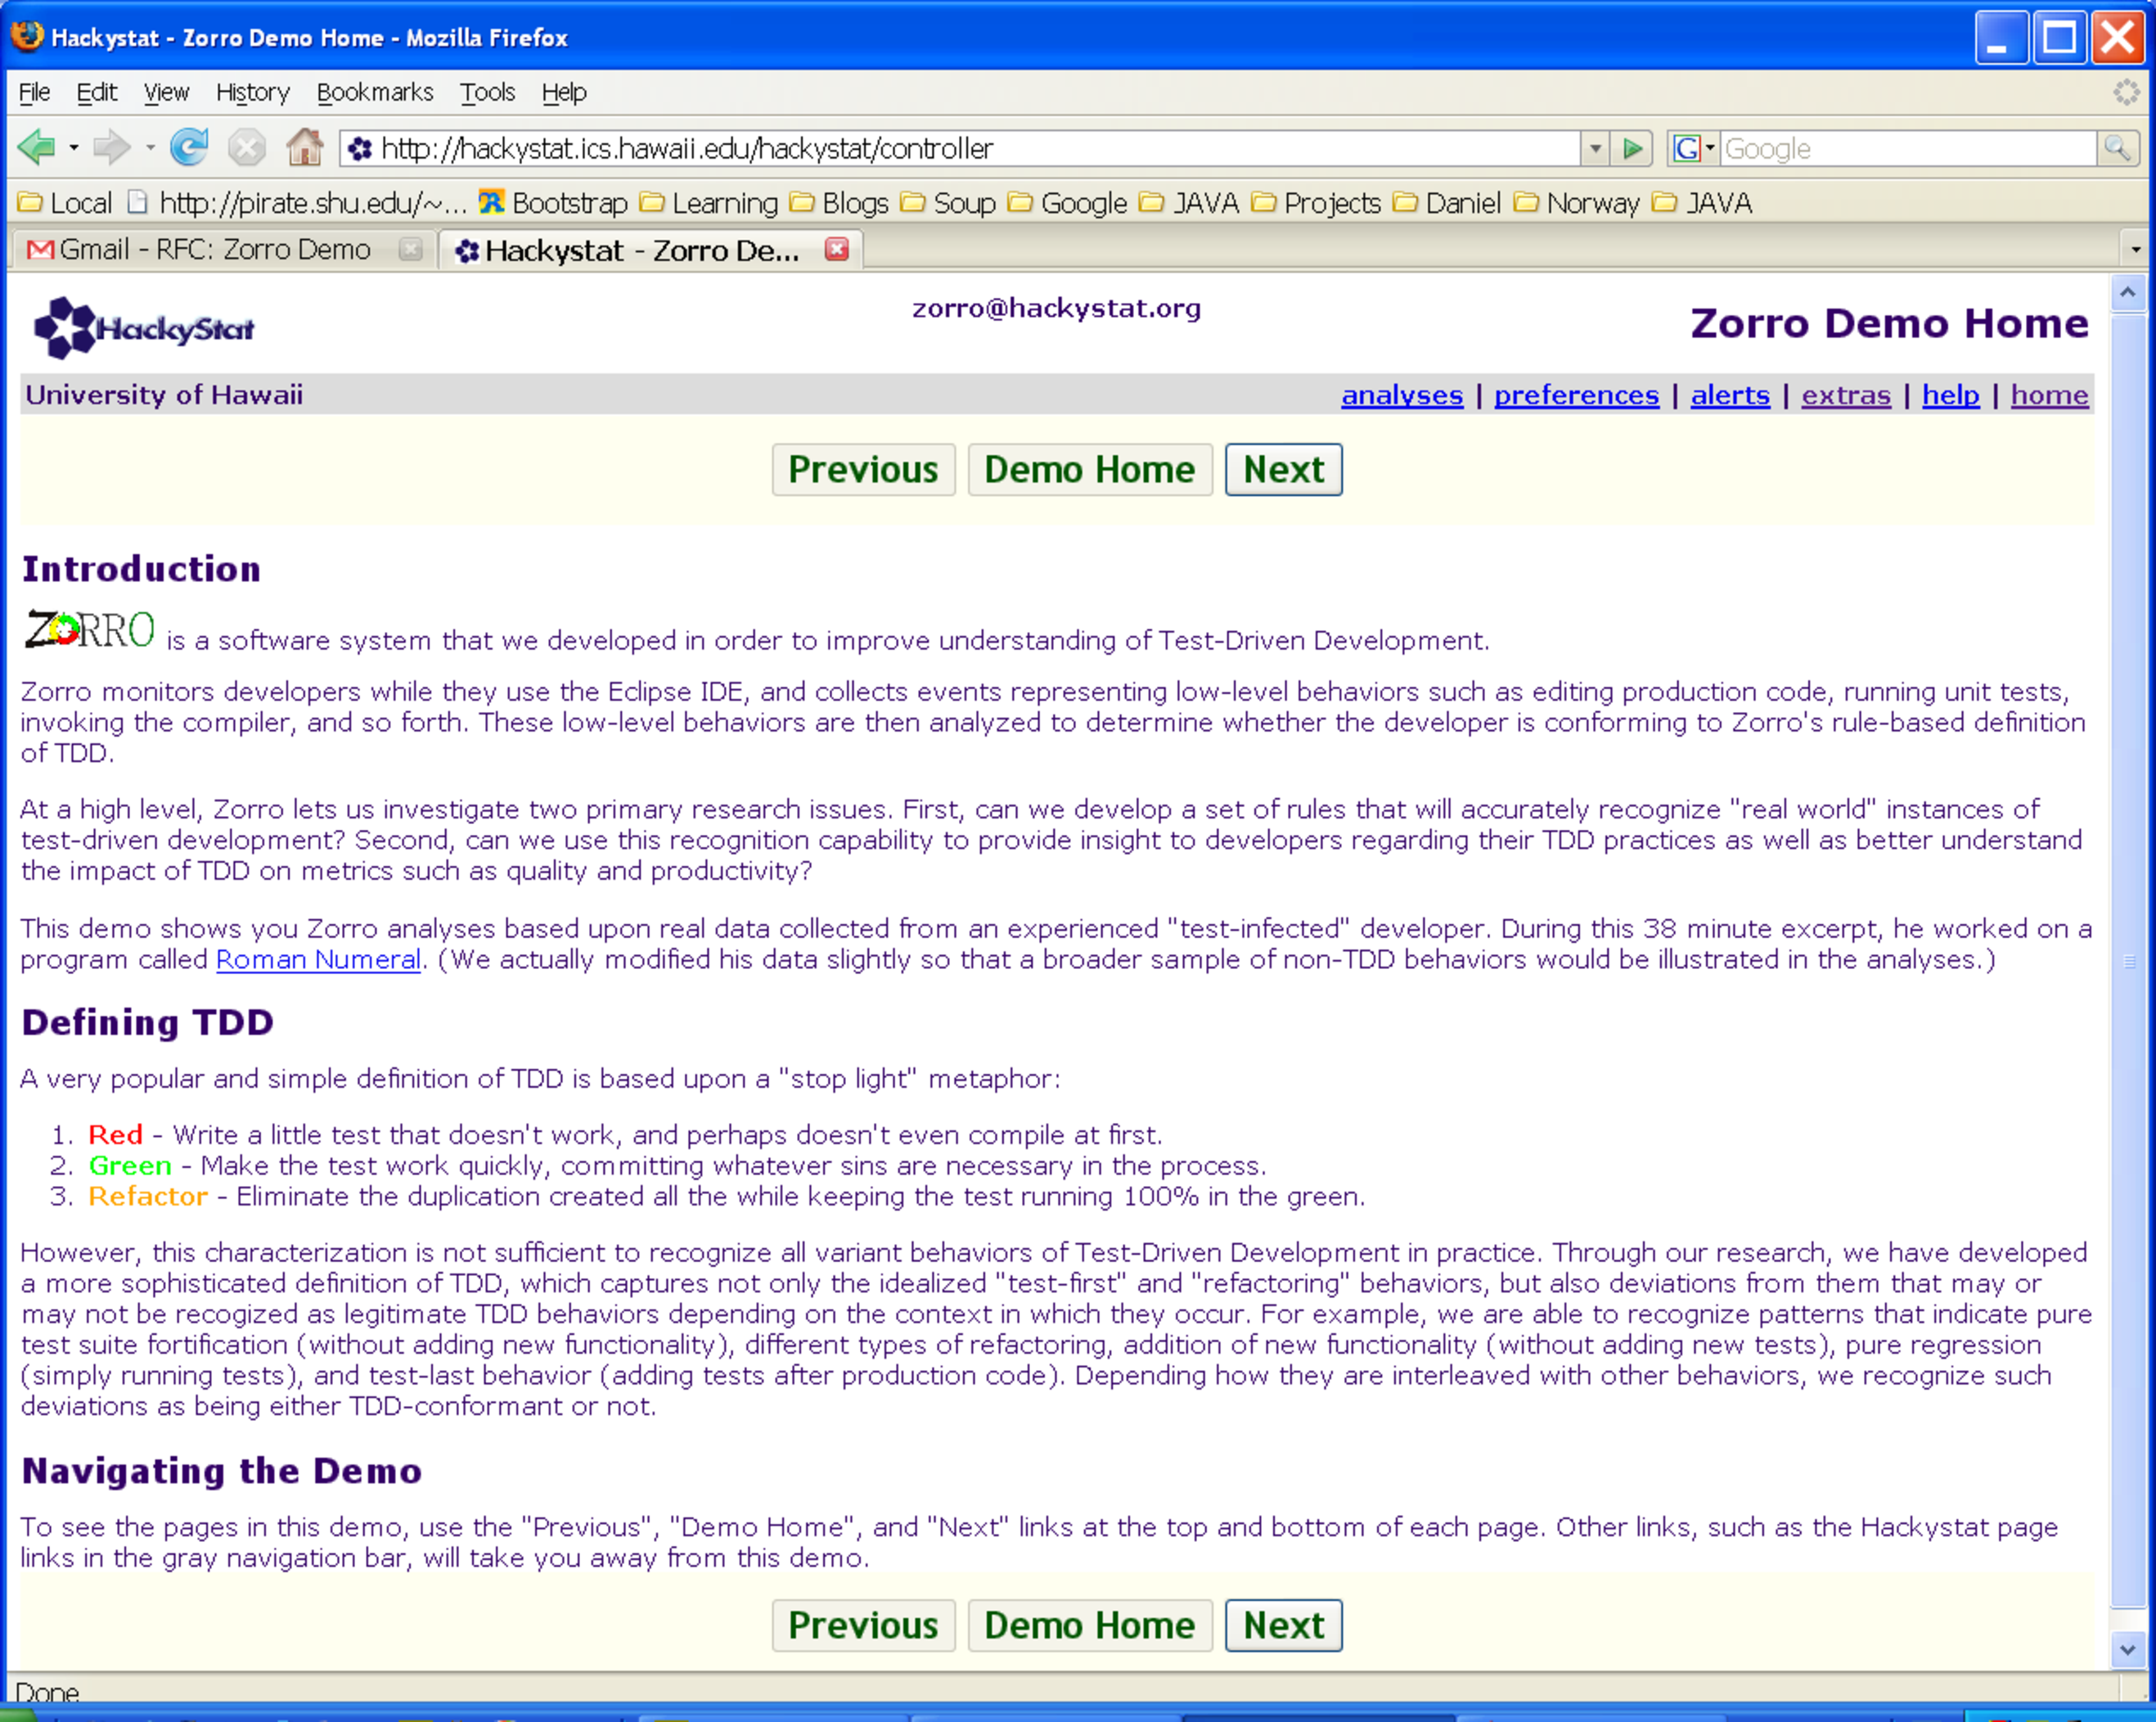
\includegraphics[width=1.0\textwidth]{figs/ZorroDemo}
  \caption{Zorro Demo Wizard}
  \label{fig:ZorroDemo}
\end{figure}

\newpage

\begin{enumerate}
\item{\textbf{TDD Episode Inference}}

Clicking the ``Next'' button in the start page will lead users to the first analysis, ``TDD Episode Inference'' (Figure \ref{fig:ZorroDemoP1}). It provides a view for end users to understand how Zorro infers compliance to TDD using collected development activities. With this analysis, beginners can learn how to program in TDD; experienced practitioners can validate the inference rules and improve their compliance to TDD; and researchers can improve validity of their empirical studies by knowing participants' compliance to TDD. 

\begin{figure}[htbp]
  \centering
  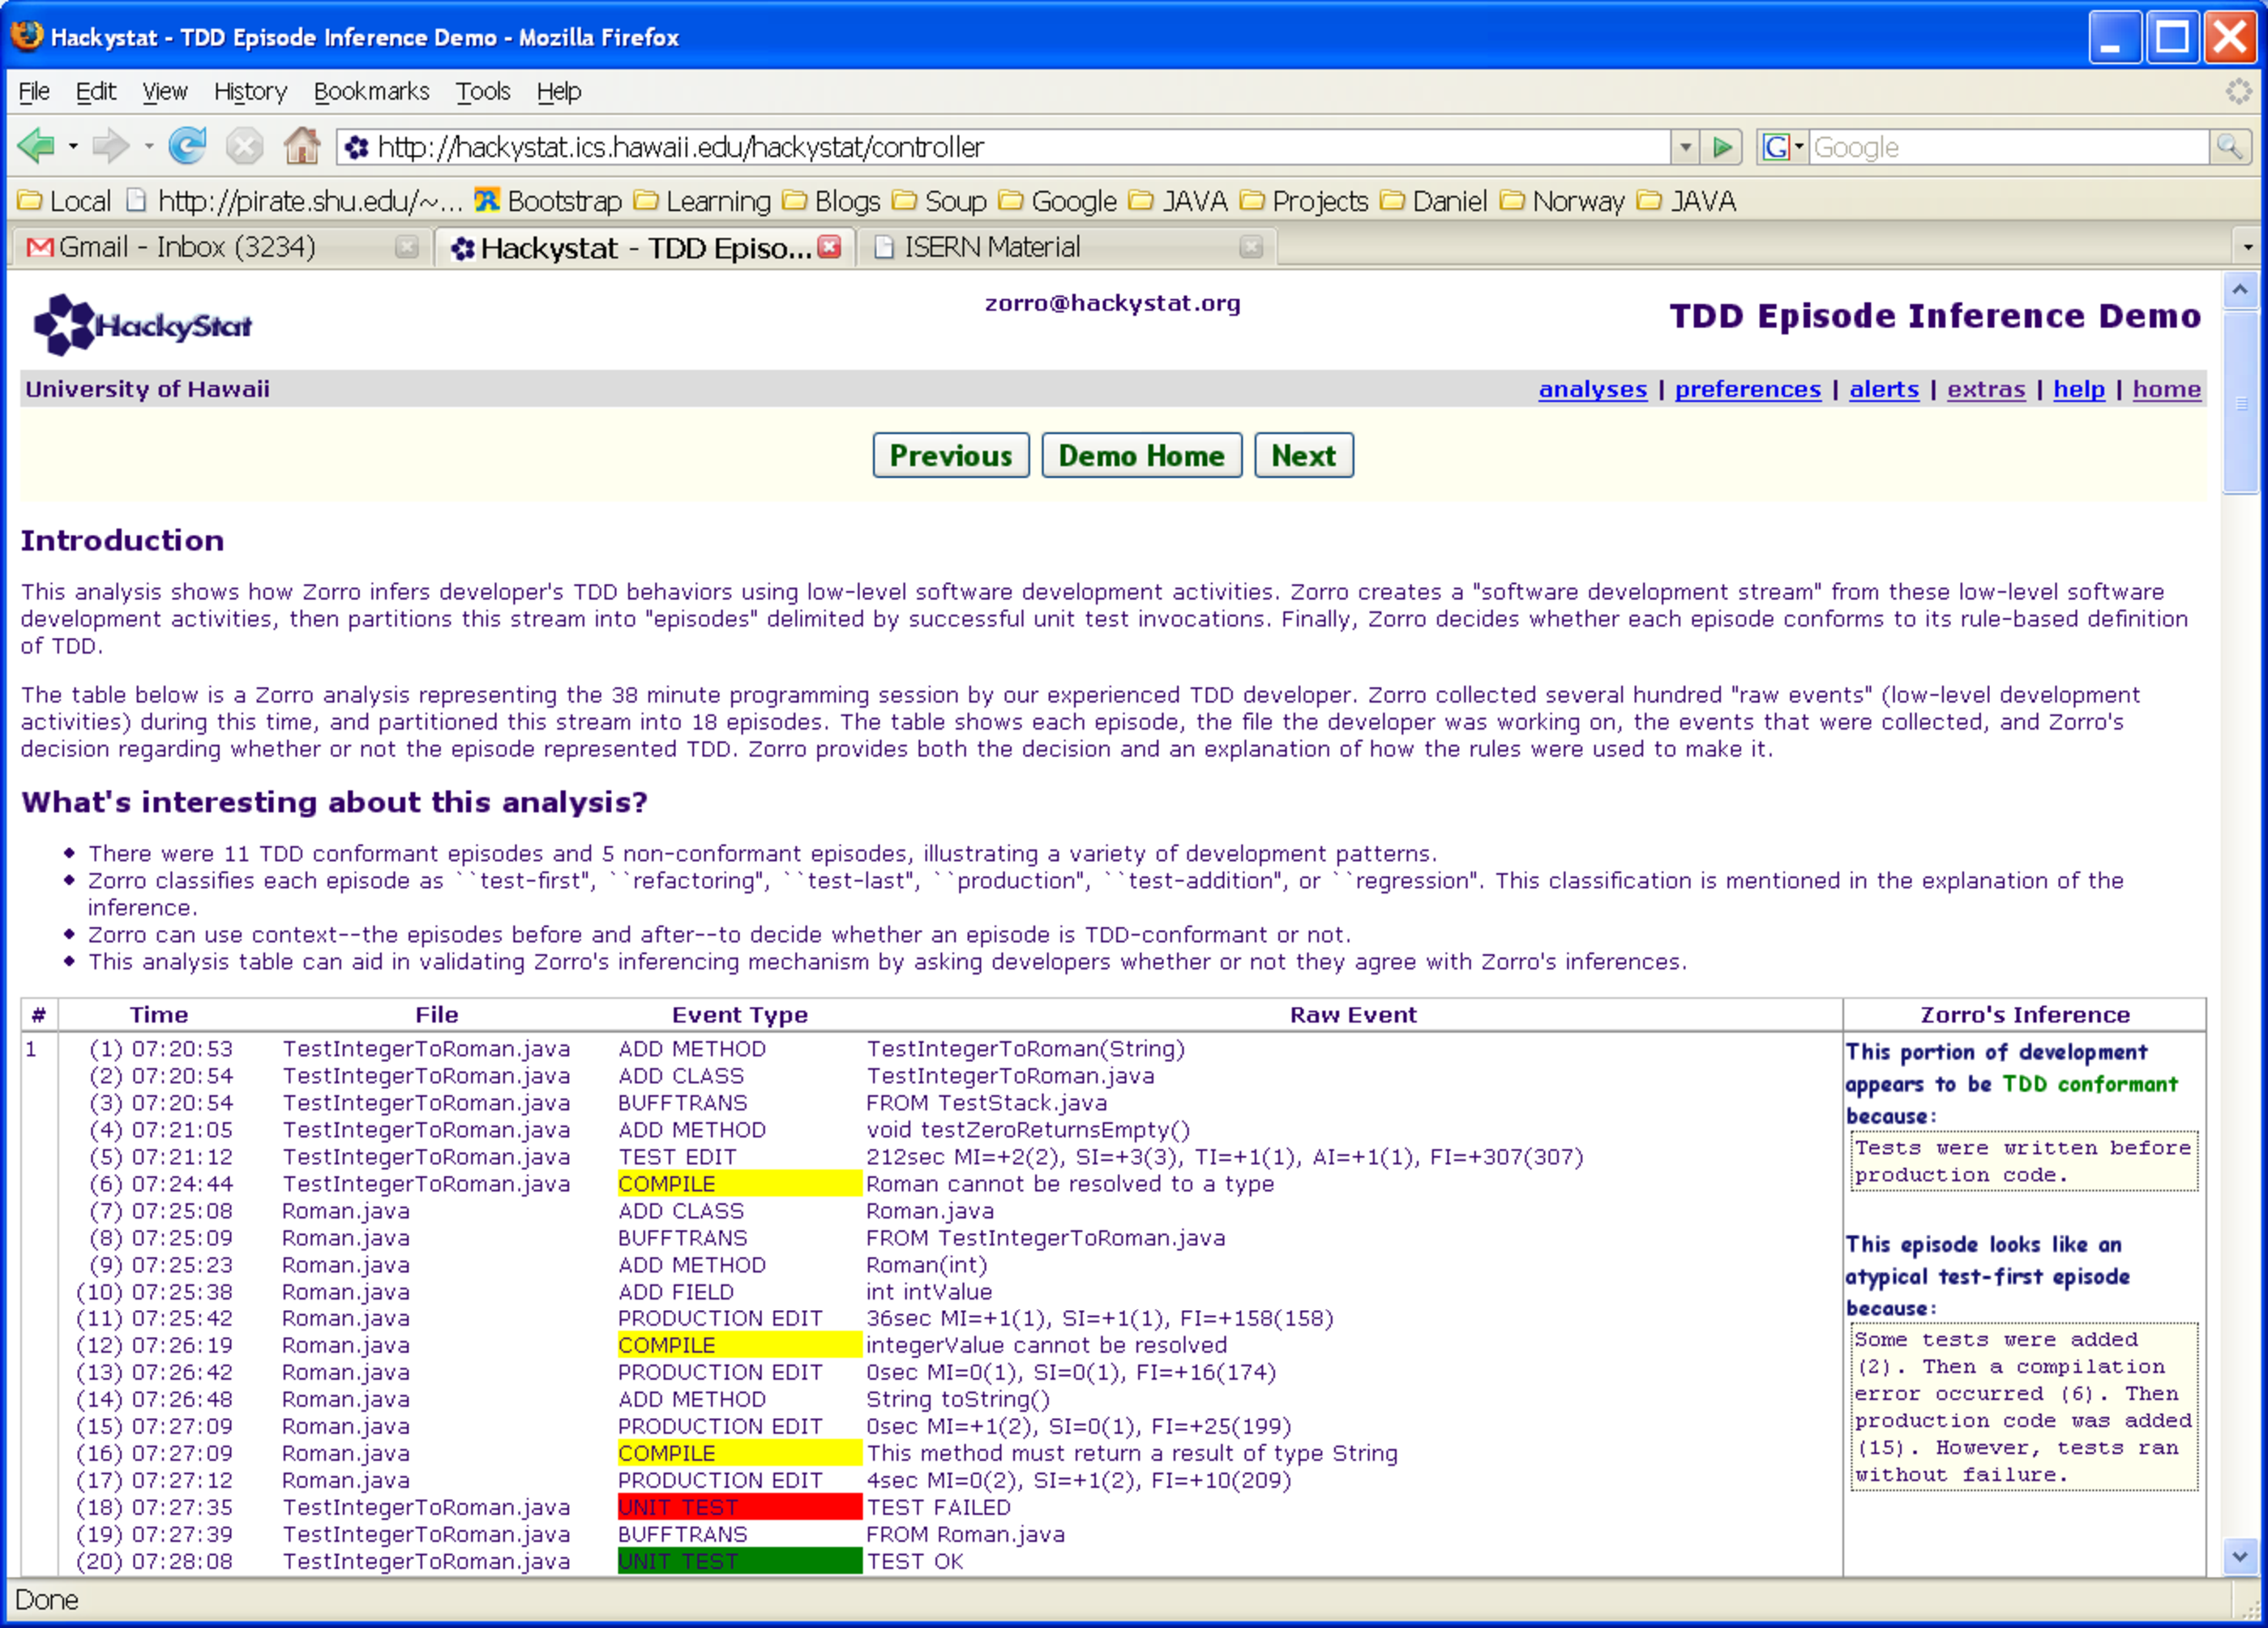
\includegraphics[width=0.9\textwidth]{figs/ZorroDemoP1}
  \caption{TDD Episode Inference Demo}
  \label{fig:ZorroDemoP1}
\end{figure}


\newpage
\item{\textbf{TDD Episode Demography}}

Following ``TDD Episode Inference'' is ``TDD Episode Demography'' that is an overview of a programming session (Figure \ref{fig:ZorroDemoP2}). It lines up all the episodes partitioned from the development stream, each of which is a box with a two-letter acronym representing the episode development behavior. With this analysis, users can inspect TDD programming sessions and look for TDD development patterns for improvement.  

\begin{figure}[htbp]
  \centering
  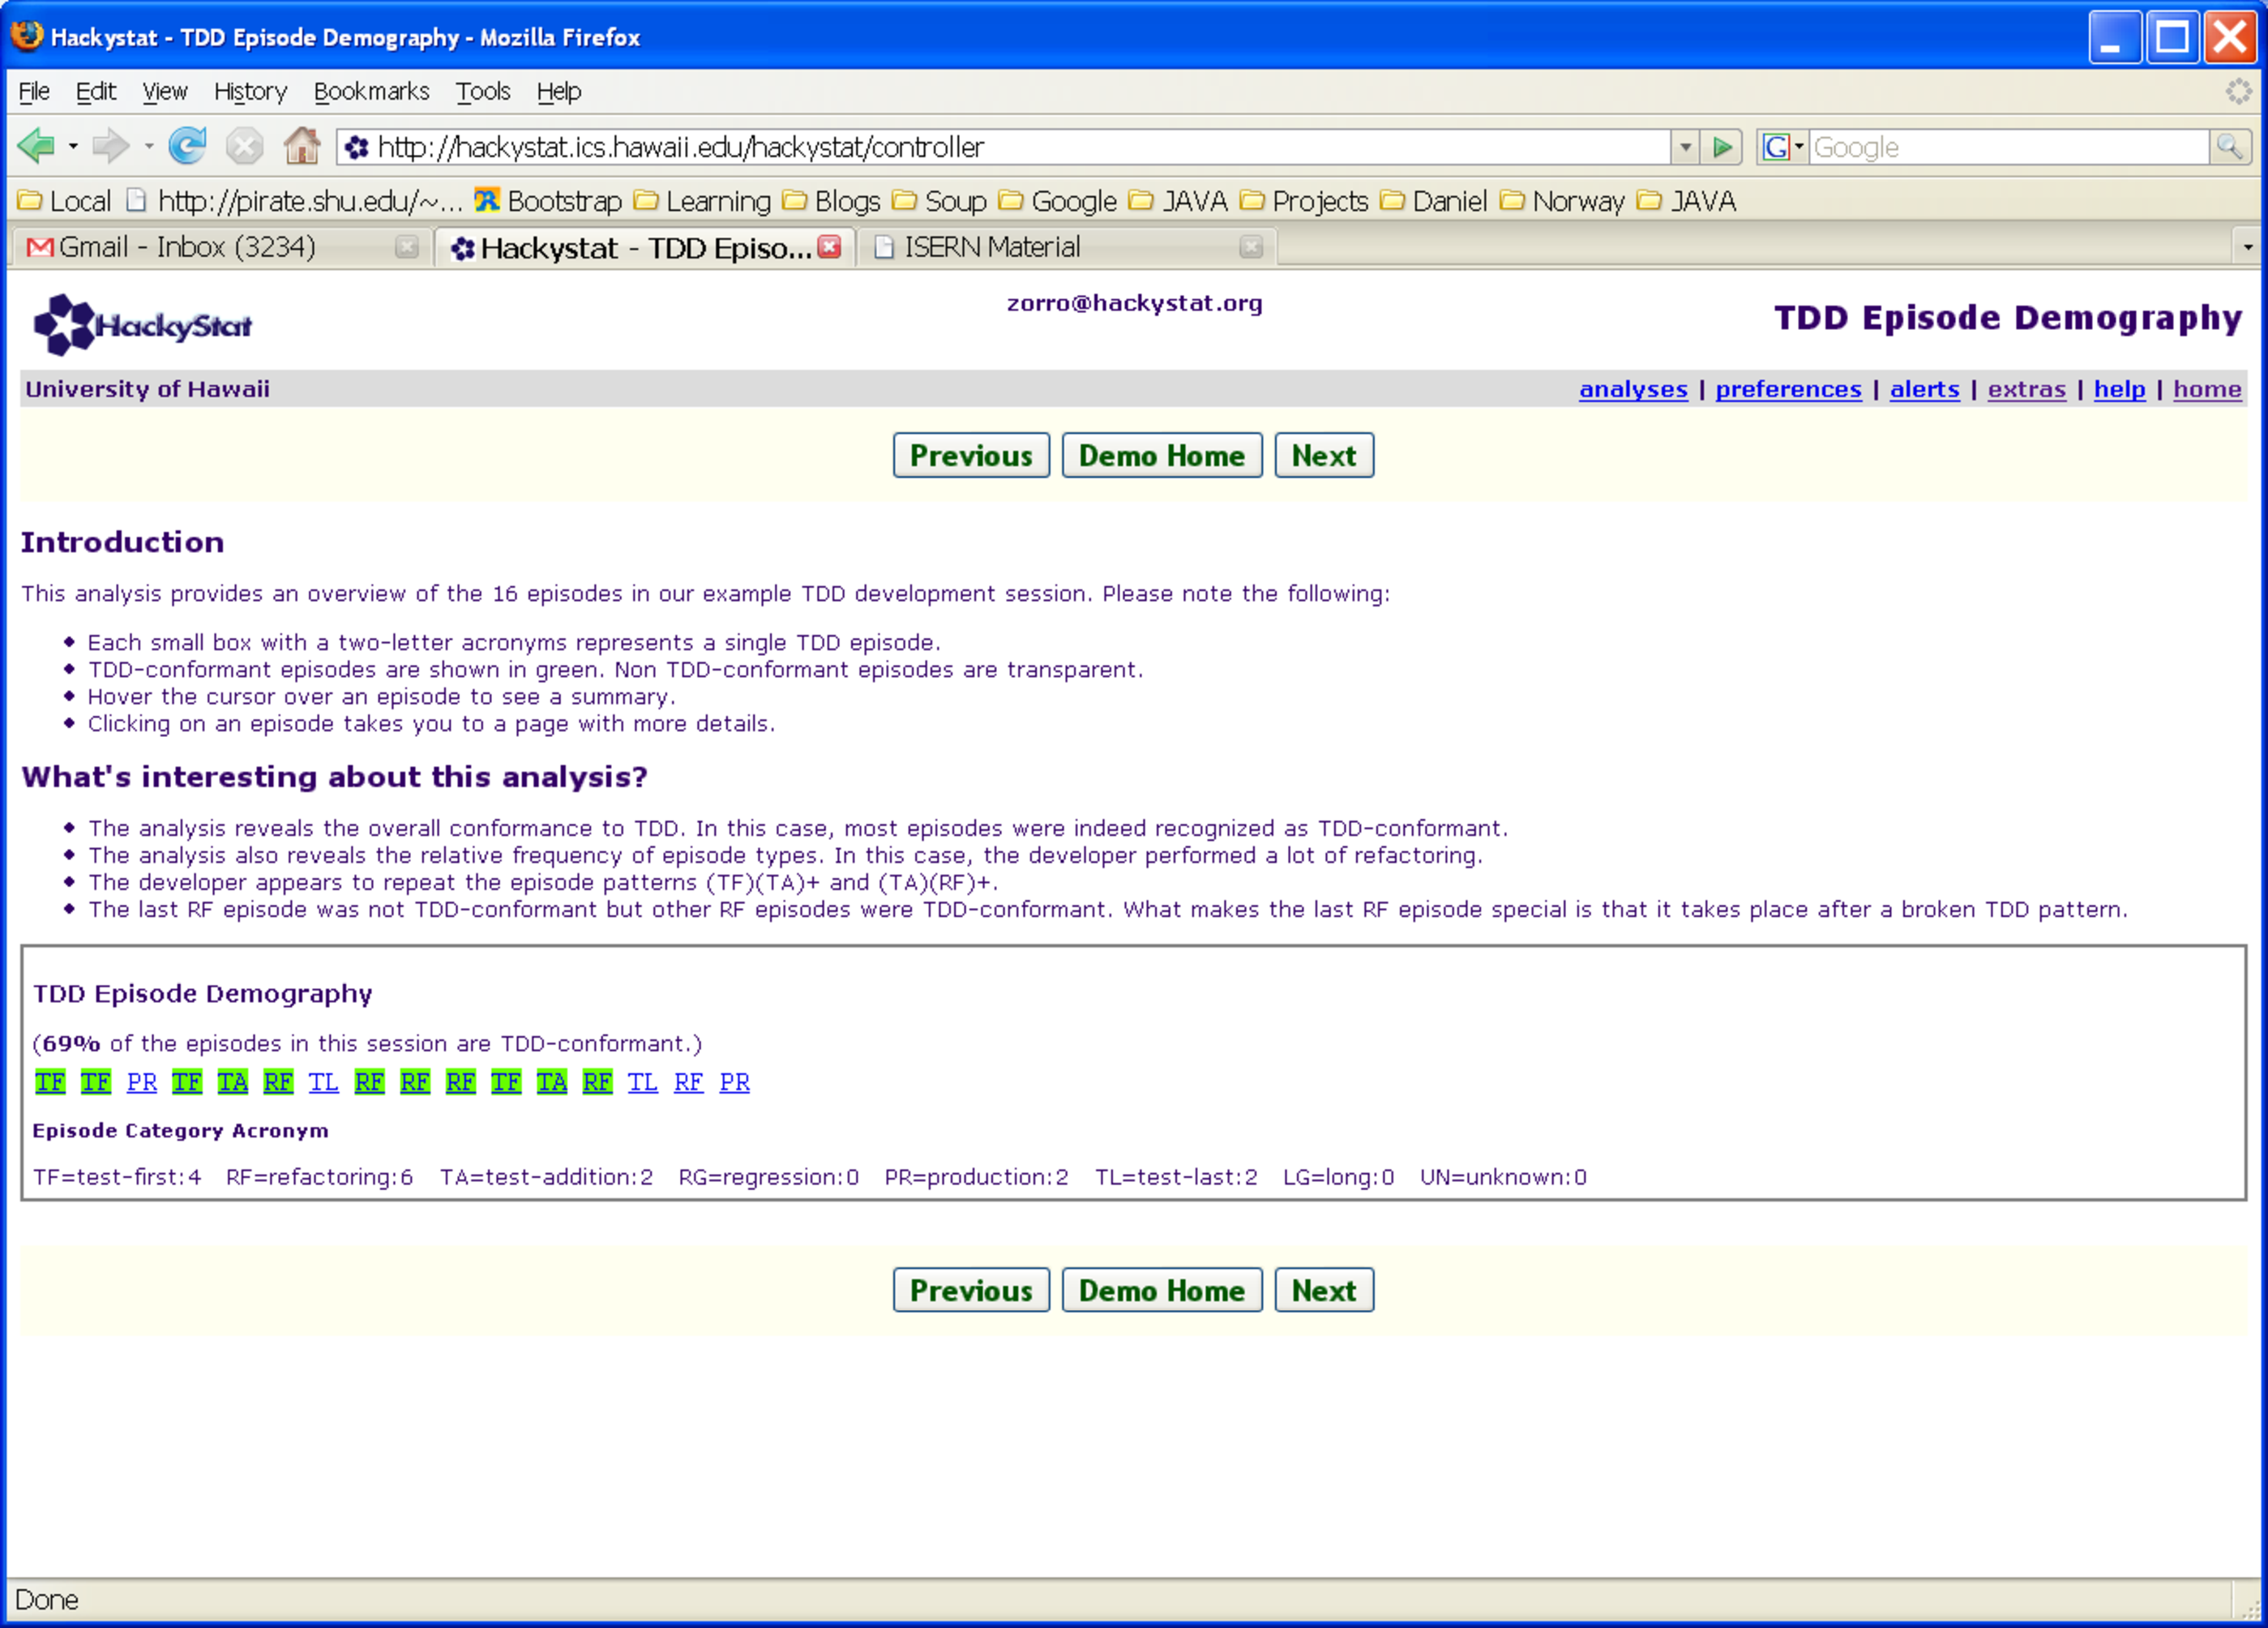
\includegraphics[width=0.9\textwidth]{figs/ZorroDemoP2}
  \caption{TDD Episode Demography}
  \label{fig:ZorroDemoP2}
\end{figure}
In addition to showing overall development behaviors and compliance to TDD, this analysis can interact with the ``TDD Episode Inference'' analysis. When users move mouse over a box in this analysis, a tooltip of episode synopsis will appear on the screen next to the mouse cursor (Figure \ref{fig:ZorroDemoP2X}), and border of the box will change to blue which indicates that it is clickable. Clicking a box will direct users to ``TDD Episode Inference'' (See Figure \ref{fig:ZorroDemoP2X2}). 
\begin{figure}[ht]
  \centering
  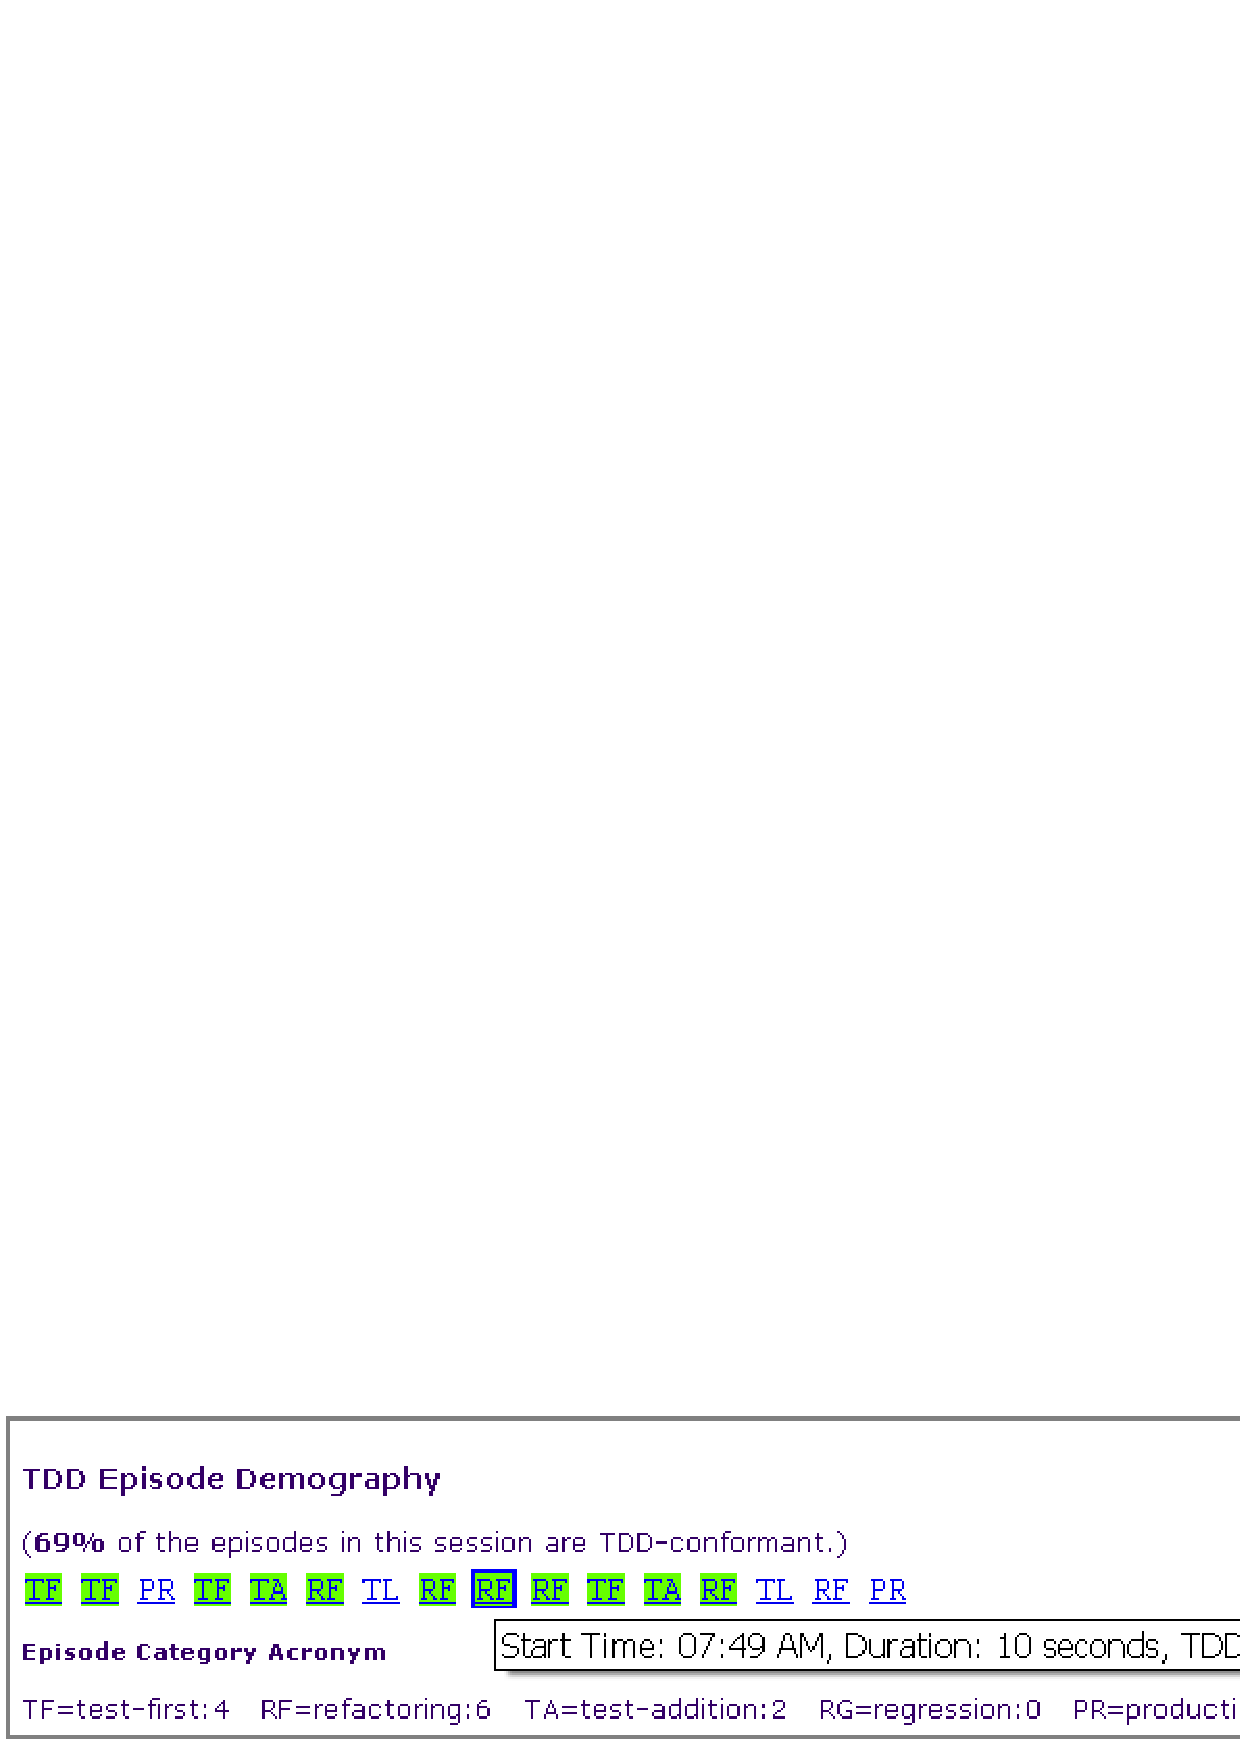
\includegraphics[width=0.9\textwidth]{figs/ZorroDemoP2X}
  \caption{Tooltip of Episode Synopsis}
  \label{fig:ZorroDemoP2X}
\end{figure}
\begin{figure}[ht]
  \centering
  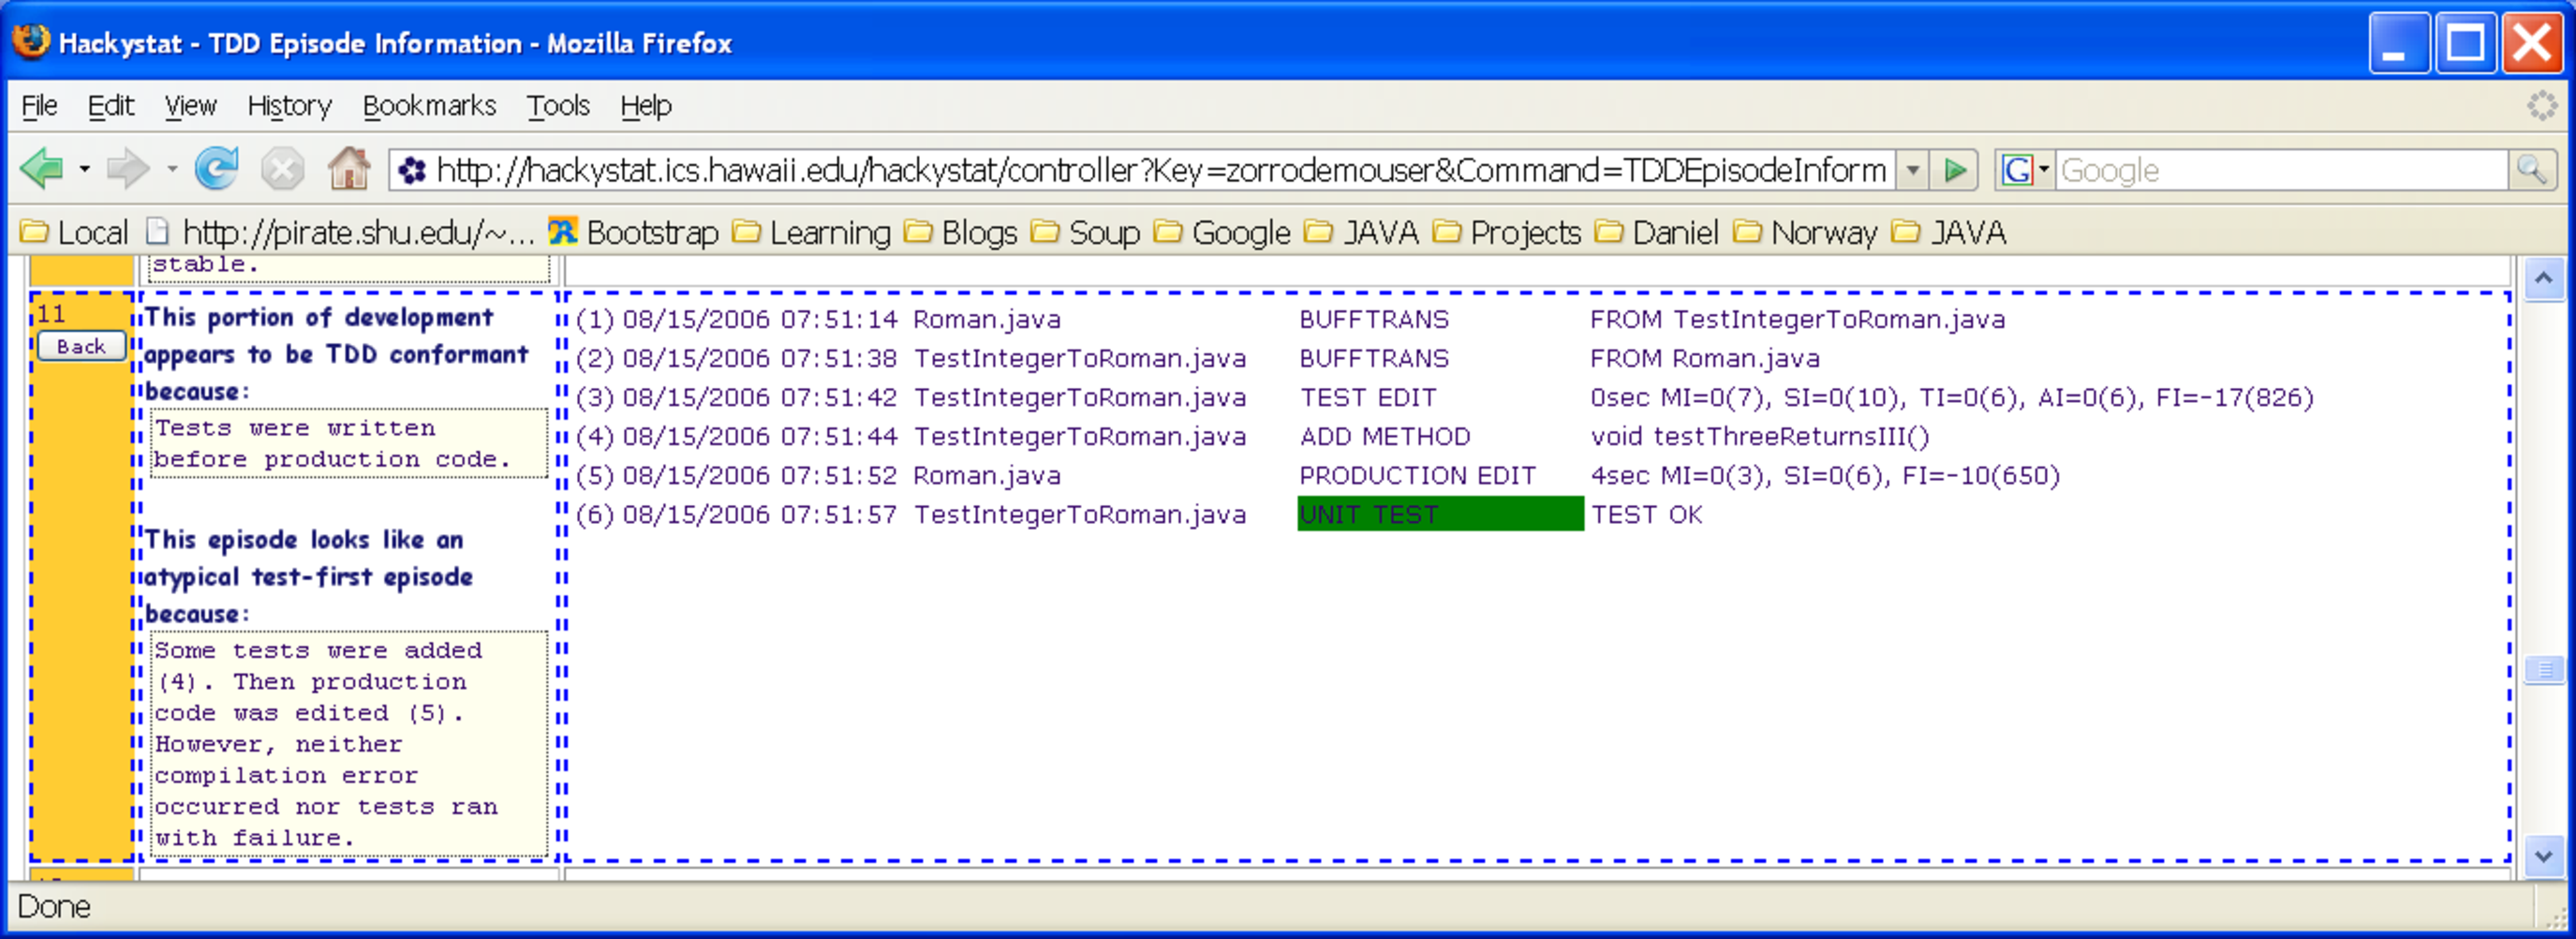
\includegraphics[width=0.9\textwidth]{figs/ZorroDemoP2X2}
  \caption{Episode Details with Back Button}
  \label{fig:ZorroDemoP2X2}
\end{figure}

\clearpage
\item{\textbf{TDD Episode T/P Ratio of Development Time}}

The third analysis is ``TDD Episode T/P Ratio of Development Time'' (Figure \ref{fig:ZorroDemoP3}). This ratio is a good indicator of TDD compliance according to \cite{Wang:04}. %Ideally, equal amount of time should be spent on test and production code if developers faithfully develop software in TDD. 
The drop of T/P ratio could be a warning signal indicating that developers might slip away from TDD. If users are not confident in Zorro's automated inference of TDD compliance, they can inspect their unit testing development activities using this analysis. For others who do not practice TDD but unit testing, this analysis can provide their dynamic unit testing behaviors. 
\begin{figure}[htbp]
  \centering
  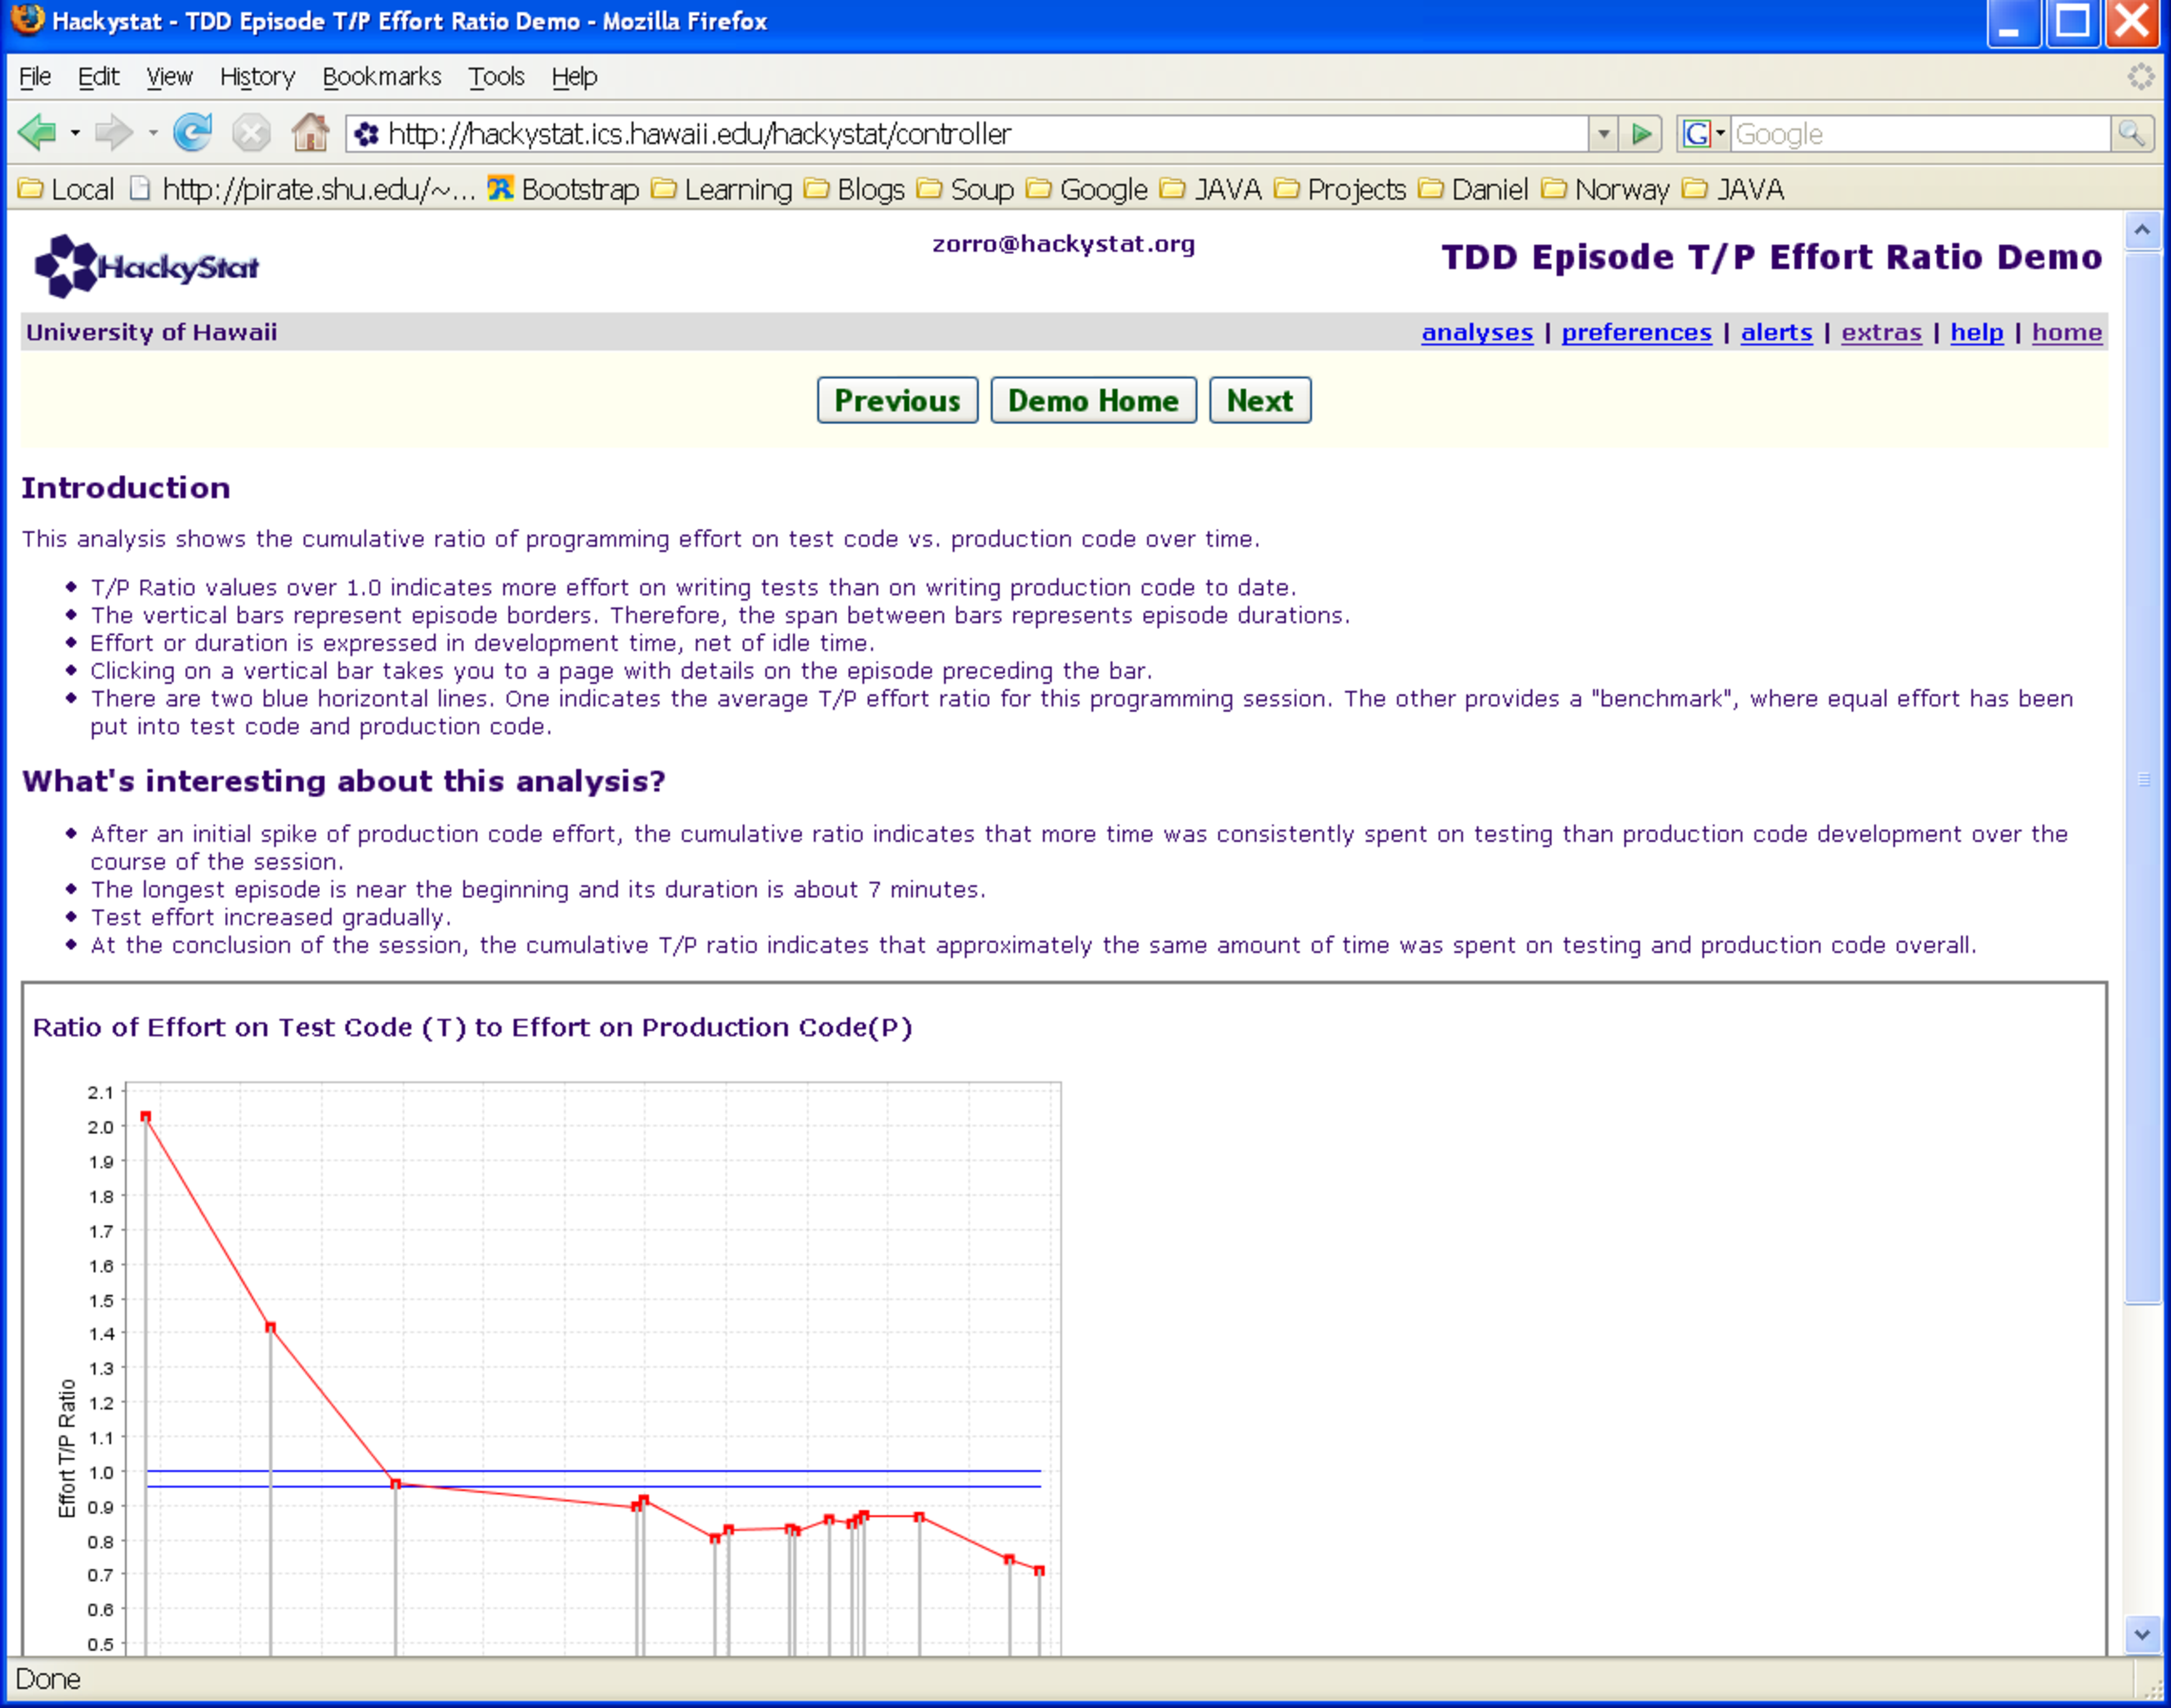
\includegraphics[width=0.9\textwidth]{figs/ZorroDemoP3}
  \caption{TDD Episode T/P Ratio of Development Time}
  \label{fig:ZorroDemoP3}
\end{figure}

\clearpage
\item{\textbf{TDD Episode T/P Ratio of Code Size}}

The fourth analysis is ``TDD Episode T/P Ratio of Code Size'' (Figure \ref{fig:ZorroDemoP4}). Similarly. it provides another metric for measuring TDD compliance. The metric of T/P ratio of code size measures the cumulative net increase of test code and production code relatives. This analysis can easily tell whether test code is written incrementally.

%However, unlike the ratio of development time, T/P ratio of code size can not be connected with the TDD compliance directly. 
\begin{figure}[htbp]
  \centering
  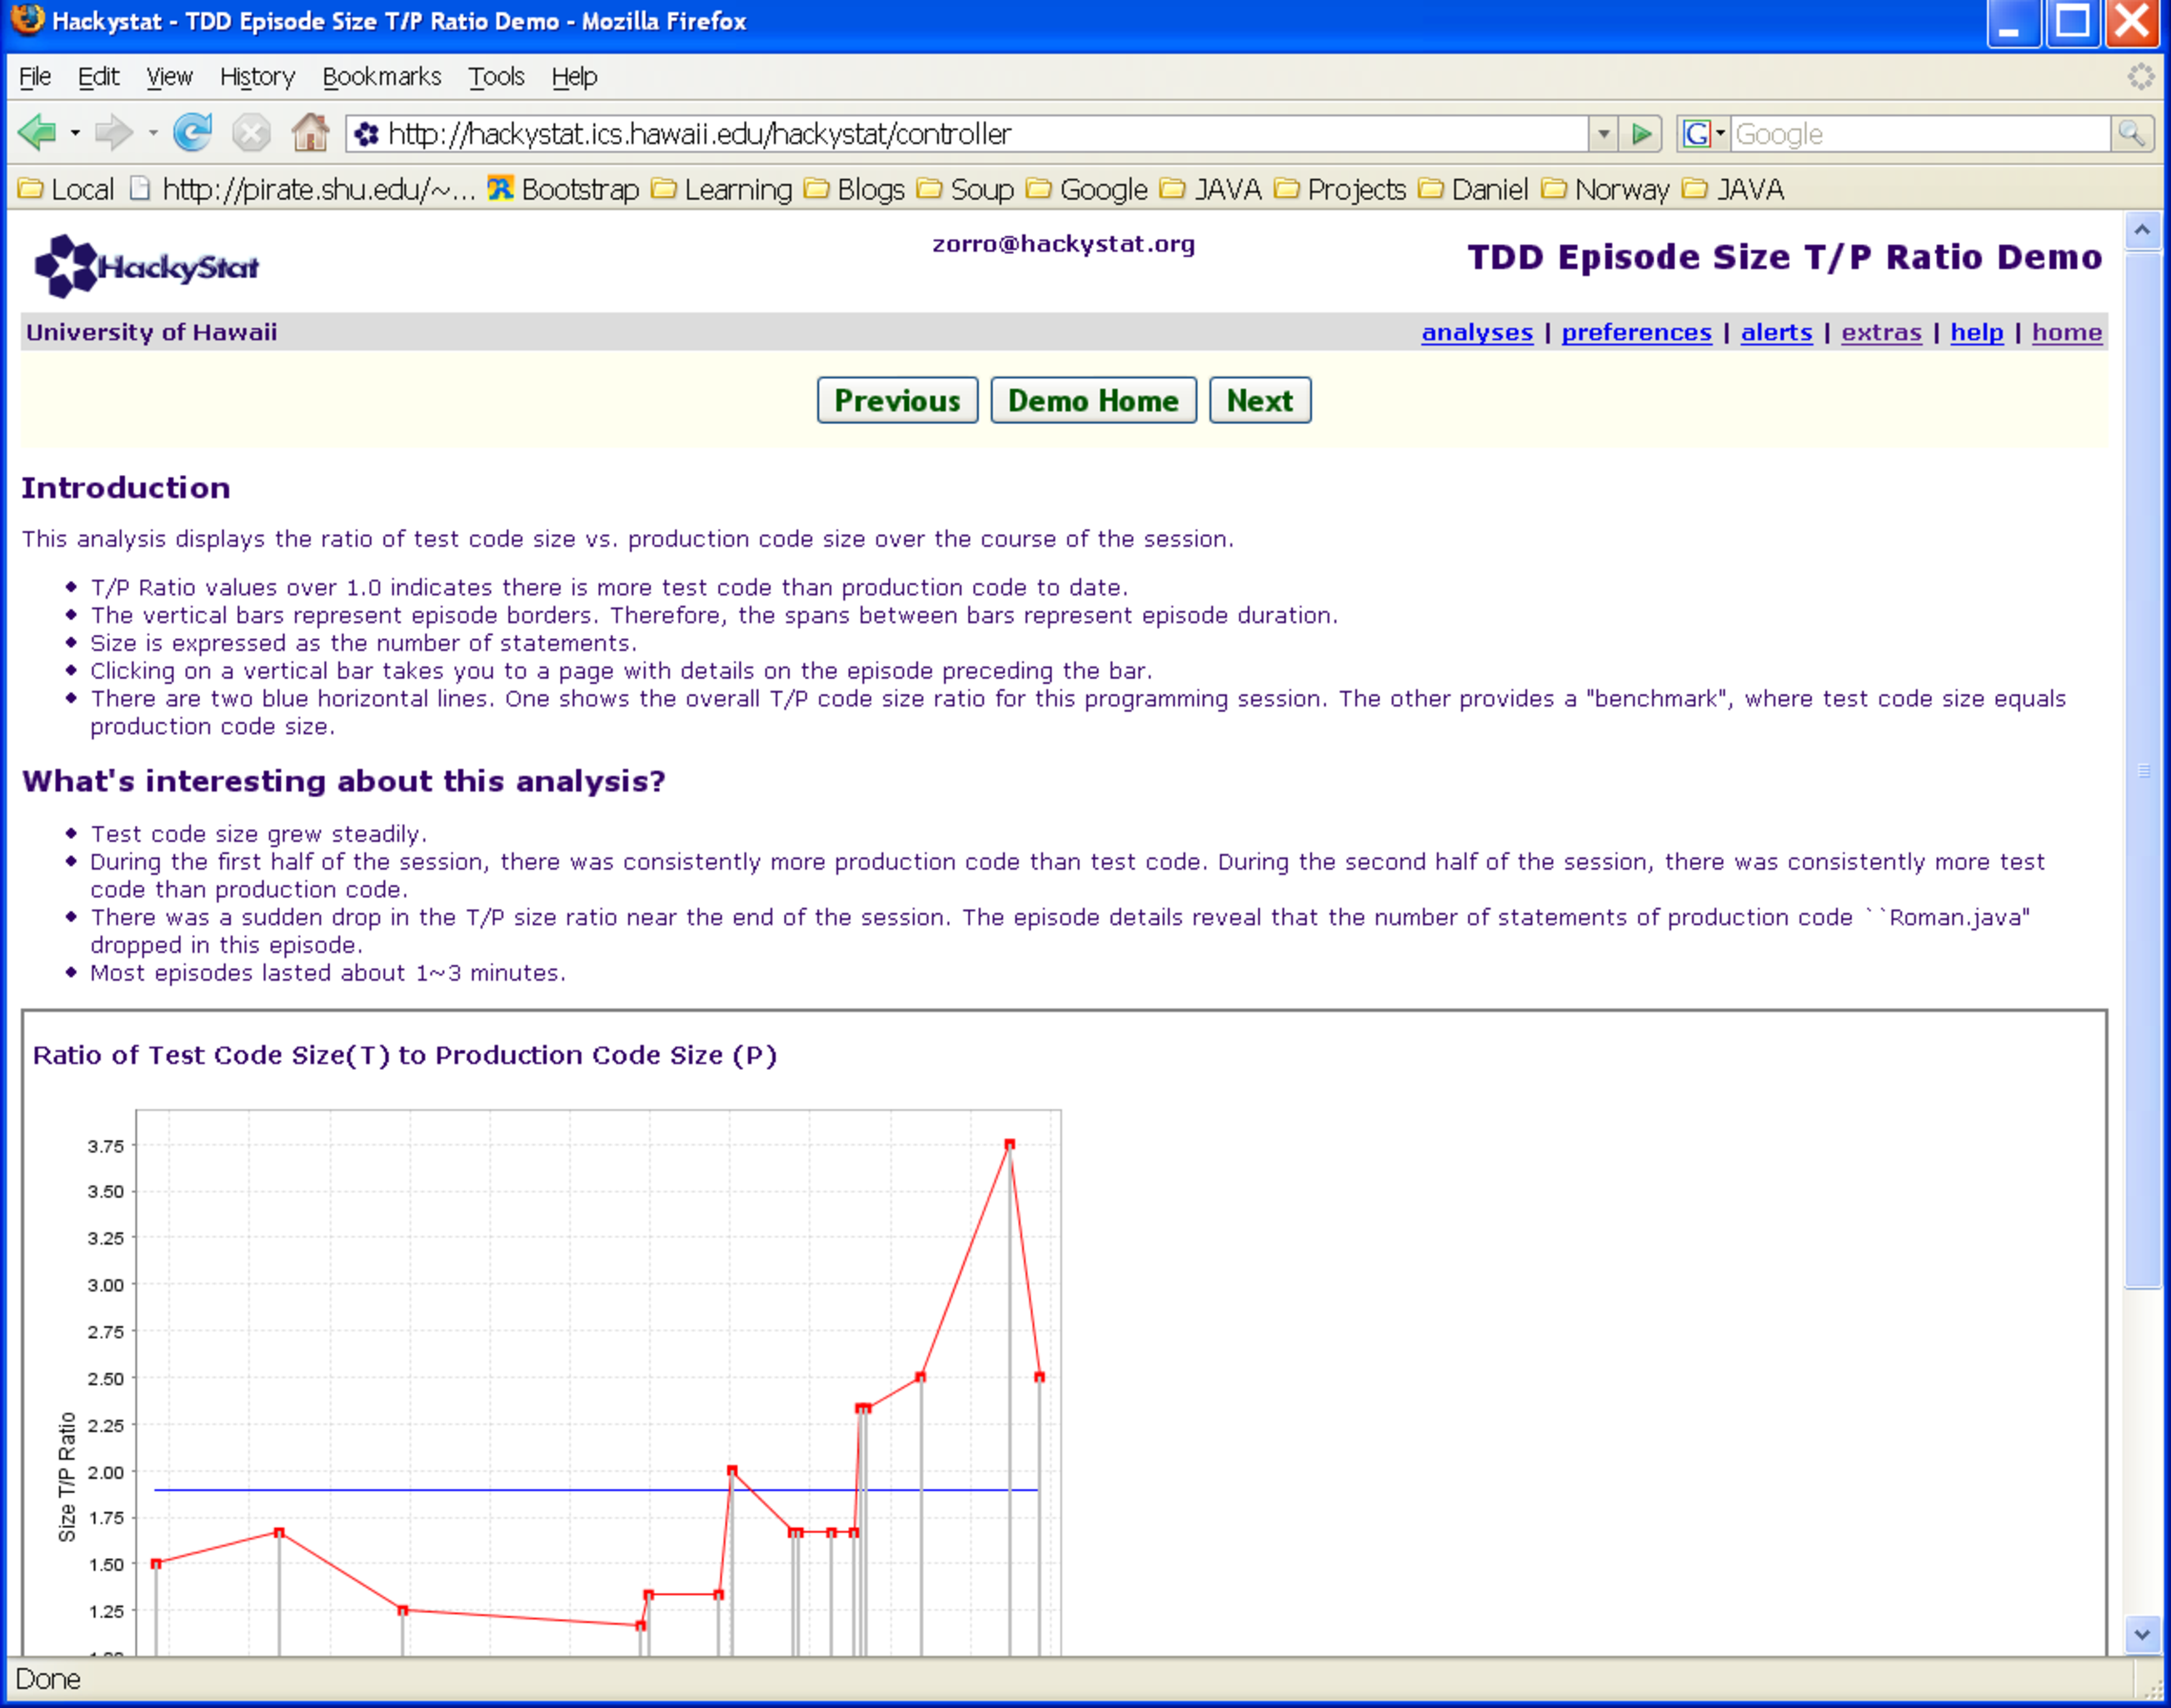
\includegraphics[width=0.9\textwidth]{figs/ZorroDemoP4}
  \caption{TDD Episode T/P Ratio of Code Size}
  \label{fig:ZorroDemoP4}
\end{figure}

%With this analysis, developers can see the moving T/P ratio over a programming session that provides information about TDD compliance too. 

\clearpage
\item{\textbf{TDD Episode Duration}}

The fifth analysis is ``TDD Episode Duration''. How often should developers invoke unit testing is a grey area of TDD. A general consensus is that an iteration of TDD should not last more than ten minutes; otherwise, the process is not agile. In Zorro, I provide the ``TDD Episode Duration'' analysis as a validation tool to observe duration of TDD iterations. It is reasonable that most episodes in TDD are short in length of duration. 
%Kent Beck stated that the occasional long iteration is not a violation to TDD \cite{Beck:03}. 
\begin{figure}[htbp]
  \centering
  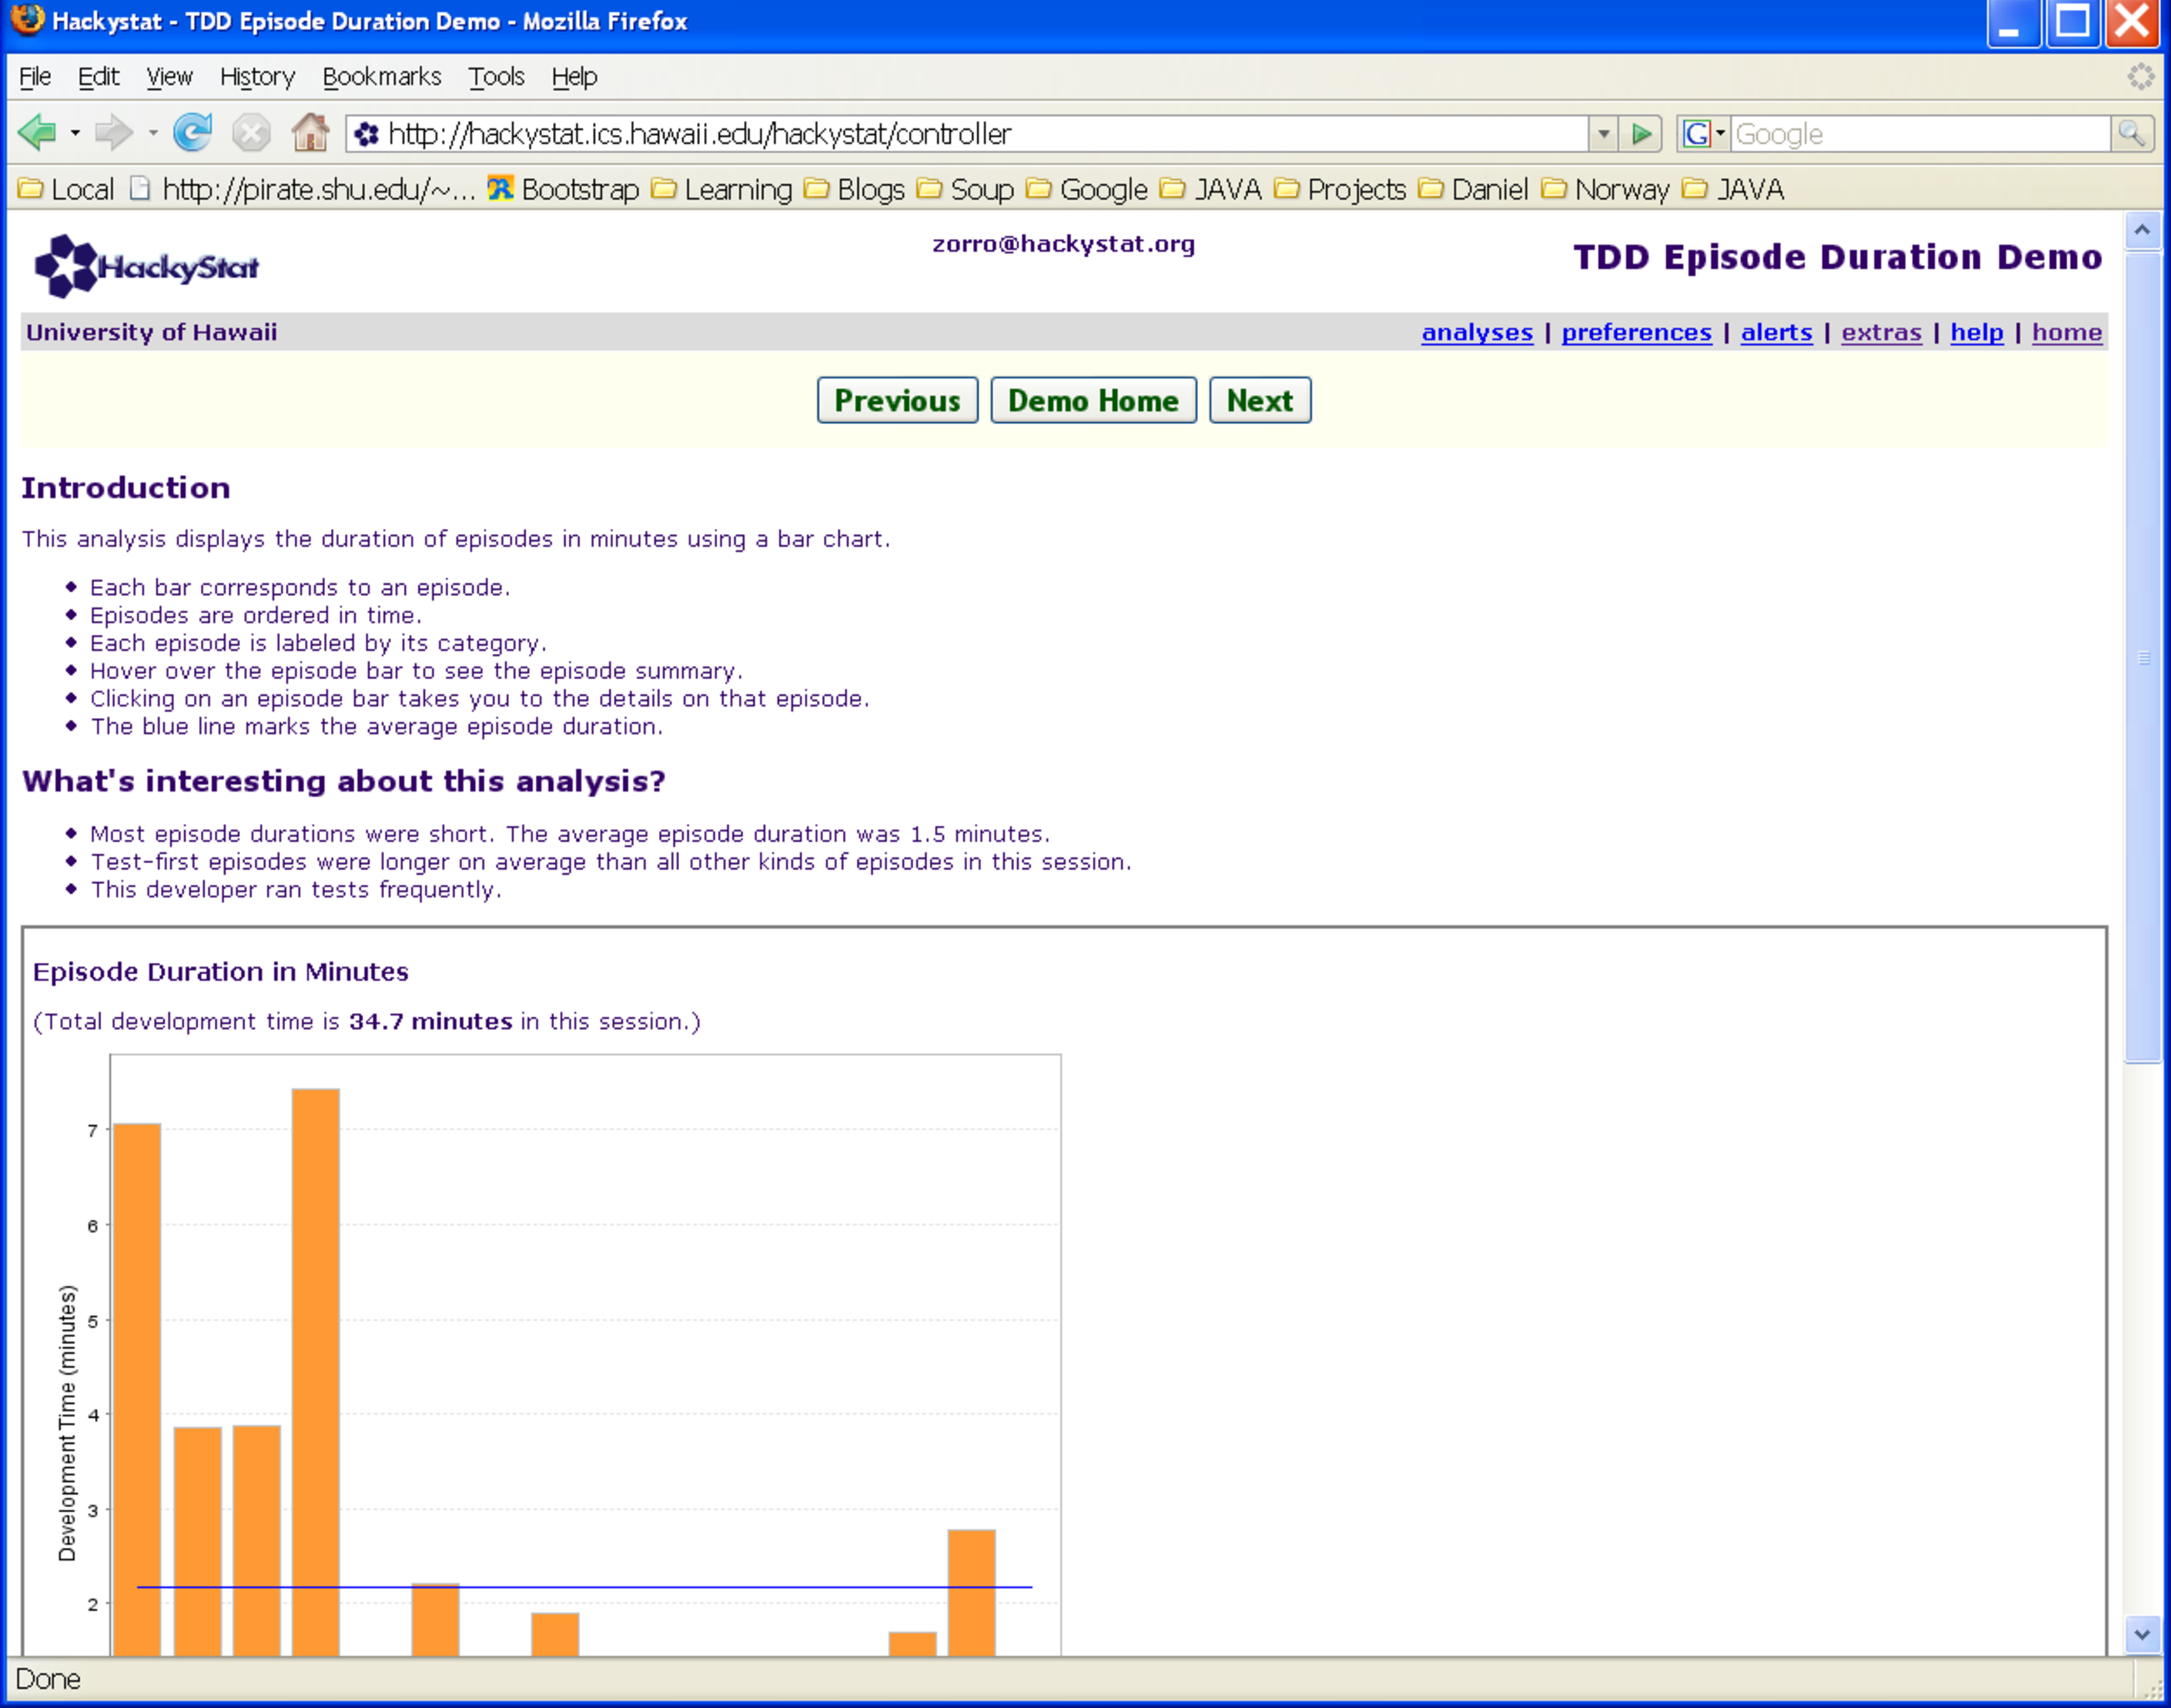
\includegraphics[width=0.9\textwidth]{figs/ZorroDemoP5}
  \caption{TDD Episode Duration}
  \label{fig:ZorroDemoP5}
\end{figure}


\newpage
\item{\textbf{TDD Episode Duration Bins}}

The last analysis is ``TDD Episode Duration Bins''. Simply as its name indicates, this analysis puts episodes into a set of bins according to their duration. Each bin defines a range of duration. In Figure \ref{fig:ZorroDemoP6}, the vertical axis is for numbers of episodes that fall into each bin. 
\begin{figure}[htbp]
  \centering
  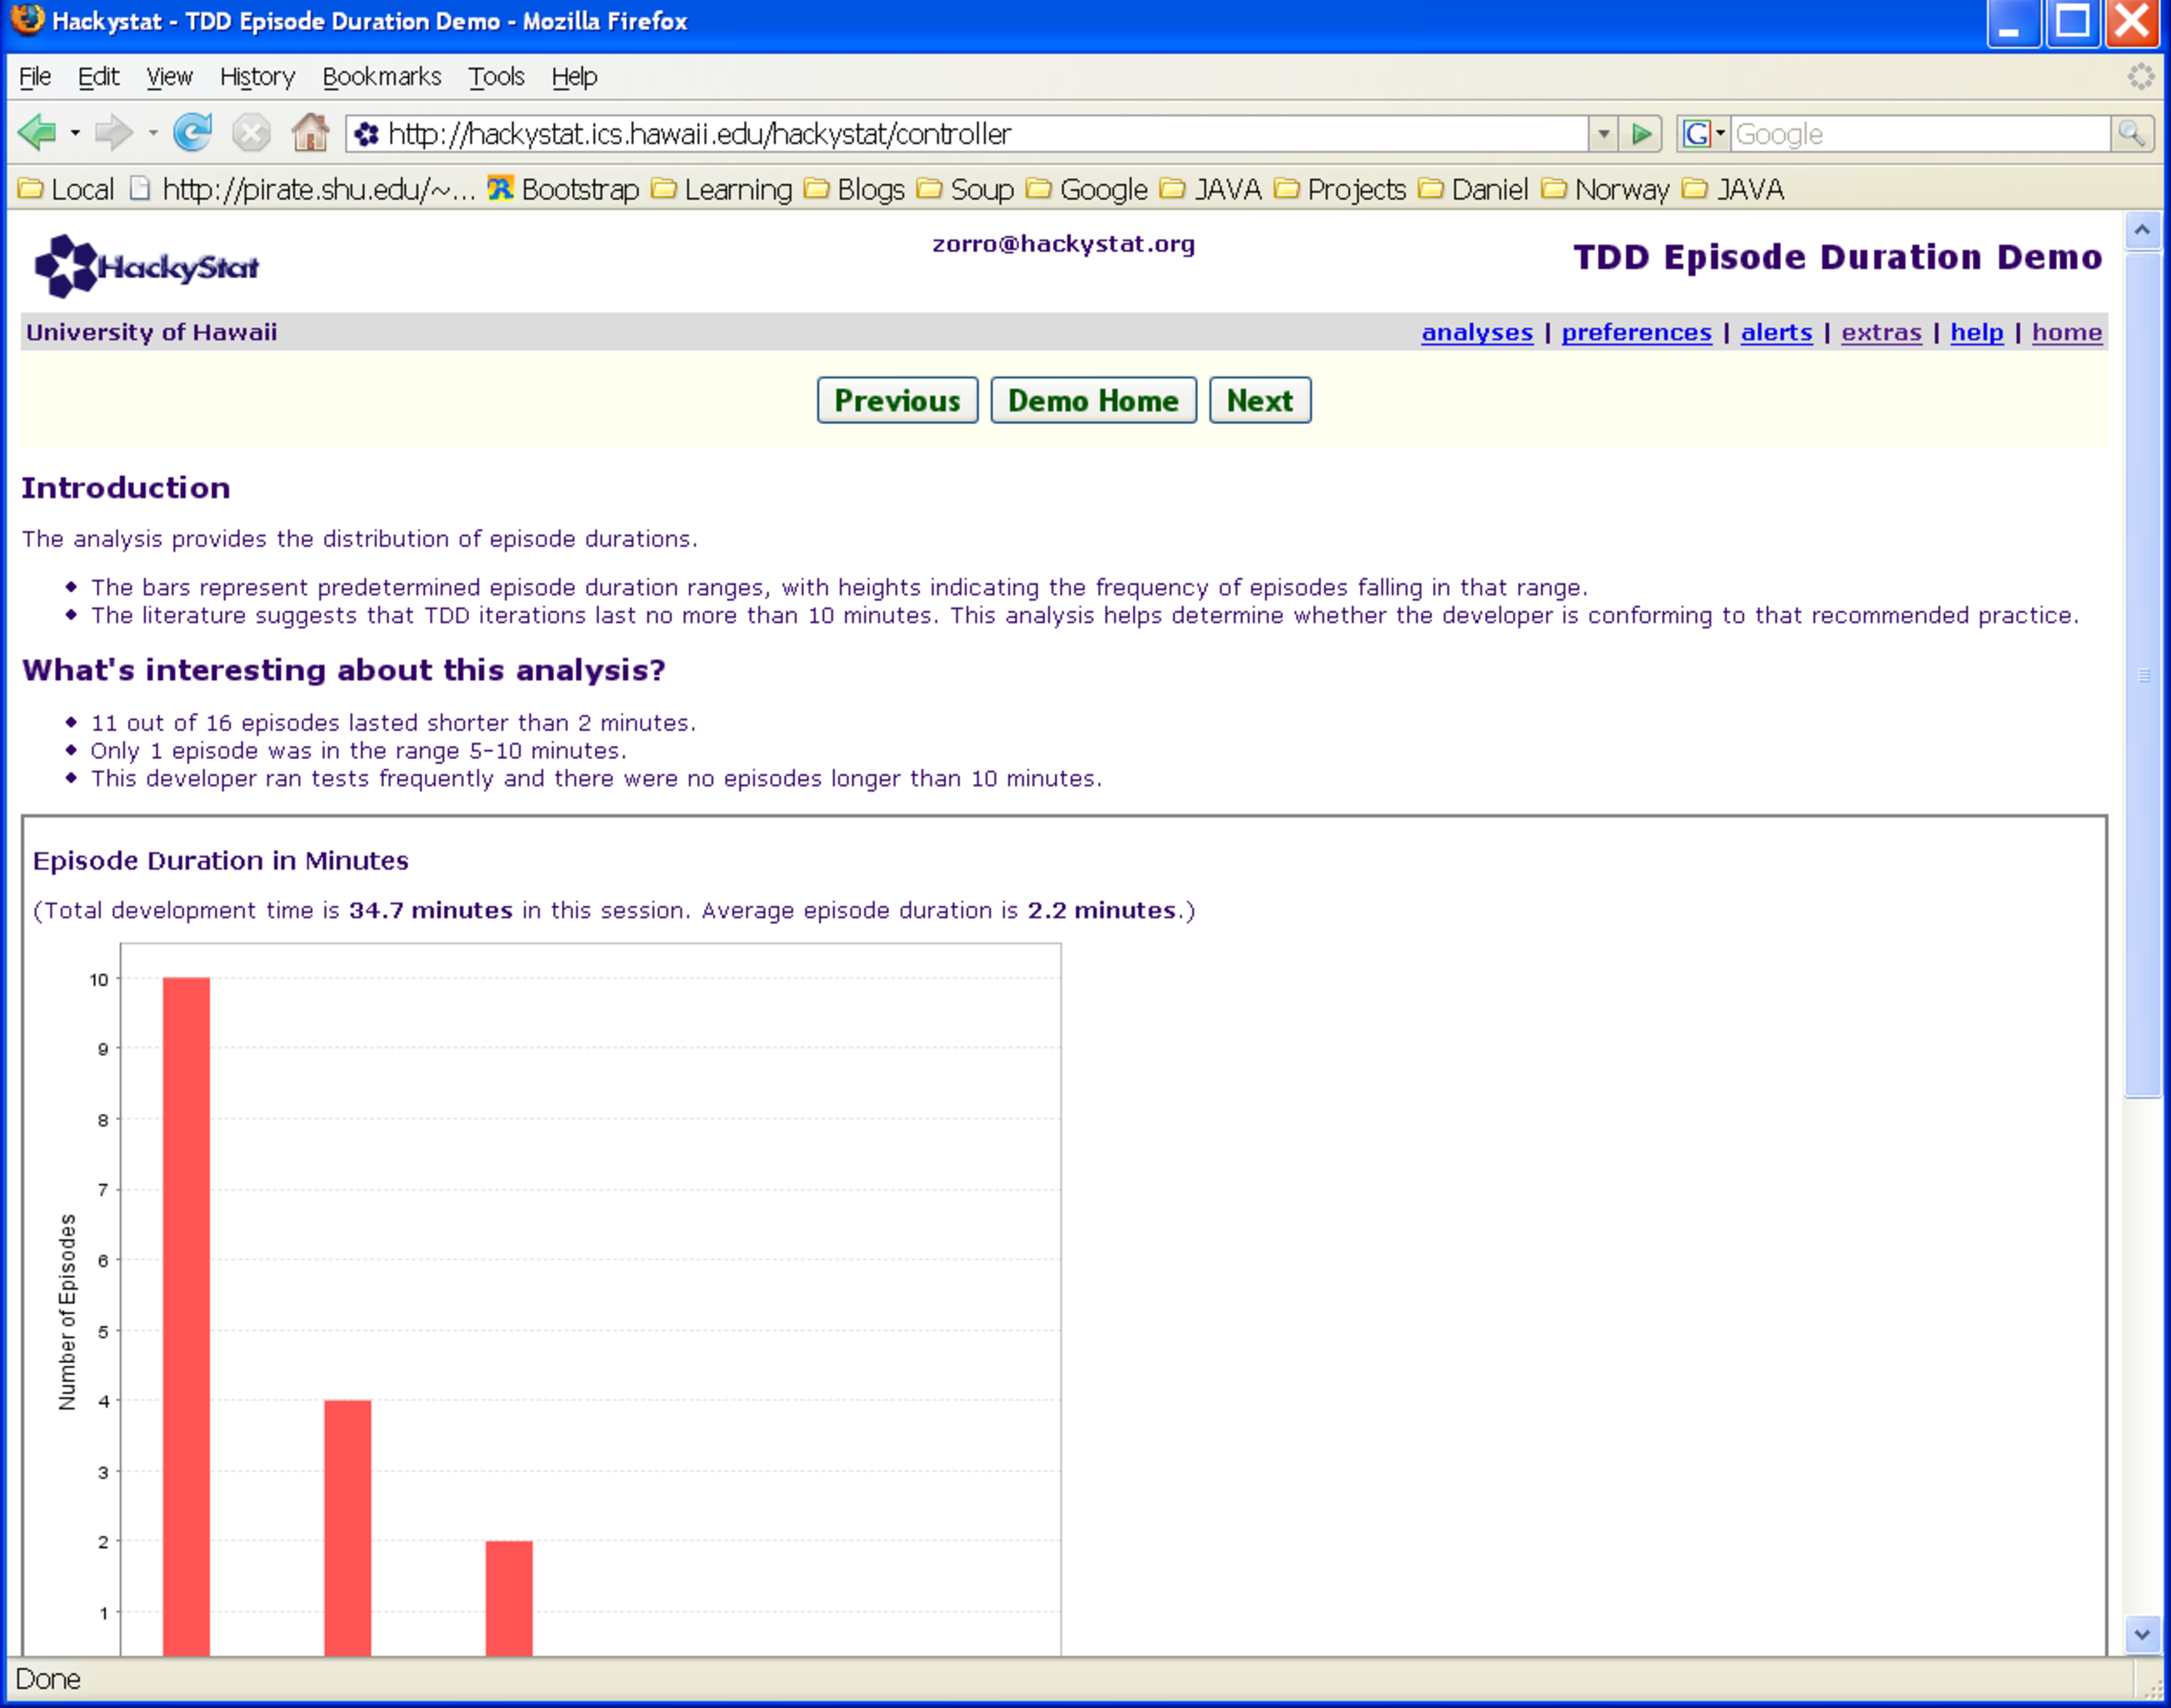
\includegraphics[width=0.9\textwidth]{figs/ZorroDemoP6}
  \caption{TDD Episode Duration Bins}
  \label{fig:ZorroDemoP6}
\end{figure}

To the TDD programming session analyzed in this demo, most episodes fell into bins of short durations according to Figure \ref{fig:ZorroDemoP6}. 

\clearpage
\item{\textbf{Zorro Demo Feedback}}

The last page of the ``Zorro Demo'' is ``Zorro Demo Feedback'' that invites readers to collaborate on studying TDD. With this demo, we targeted at three kinds of users: TDD beginners, experienced TDD practitioners, and TDD researchers. After reading information about collaborative research opportunity with us, readers can provide feedback to us using the box included in this page (Figure \ref{fig:ZorroDemoP7}). 

\begin{figure}[htbp]
  \centering
  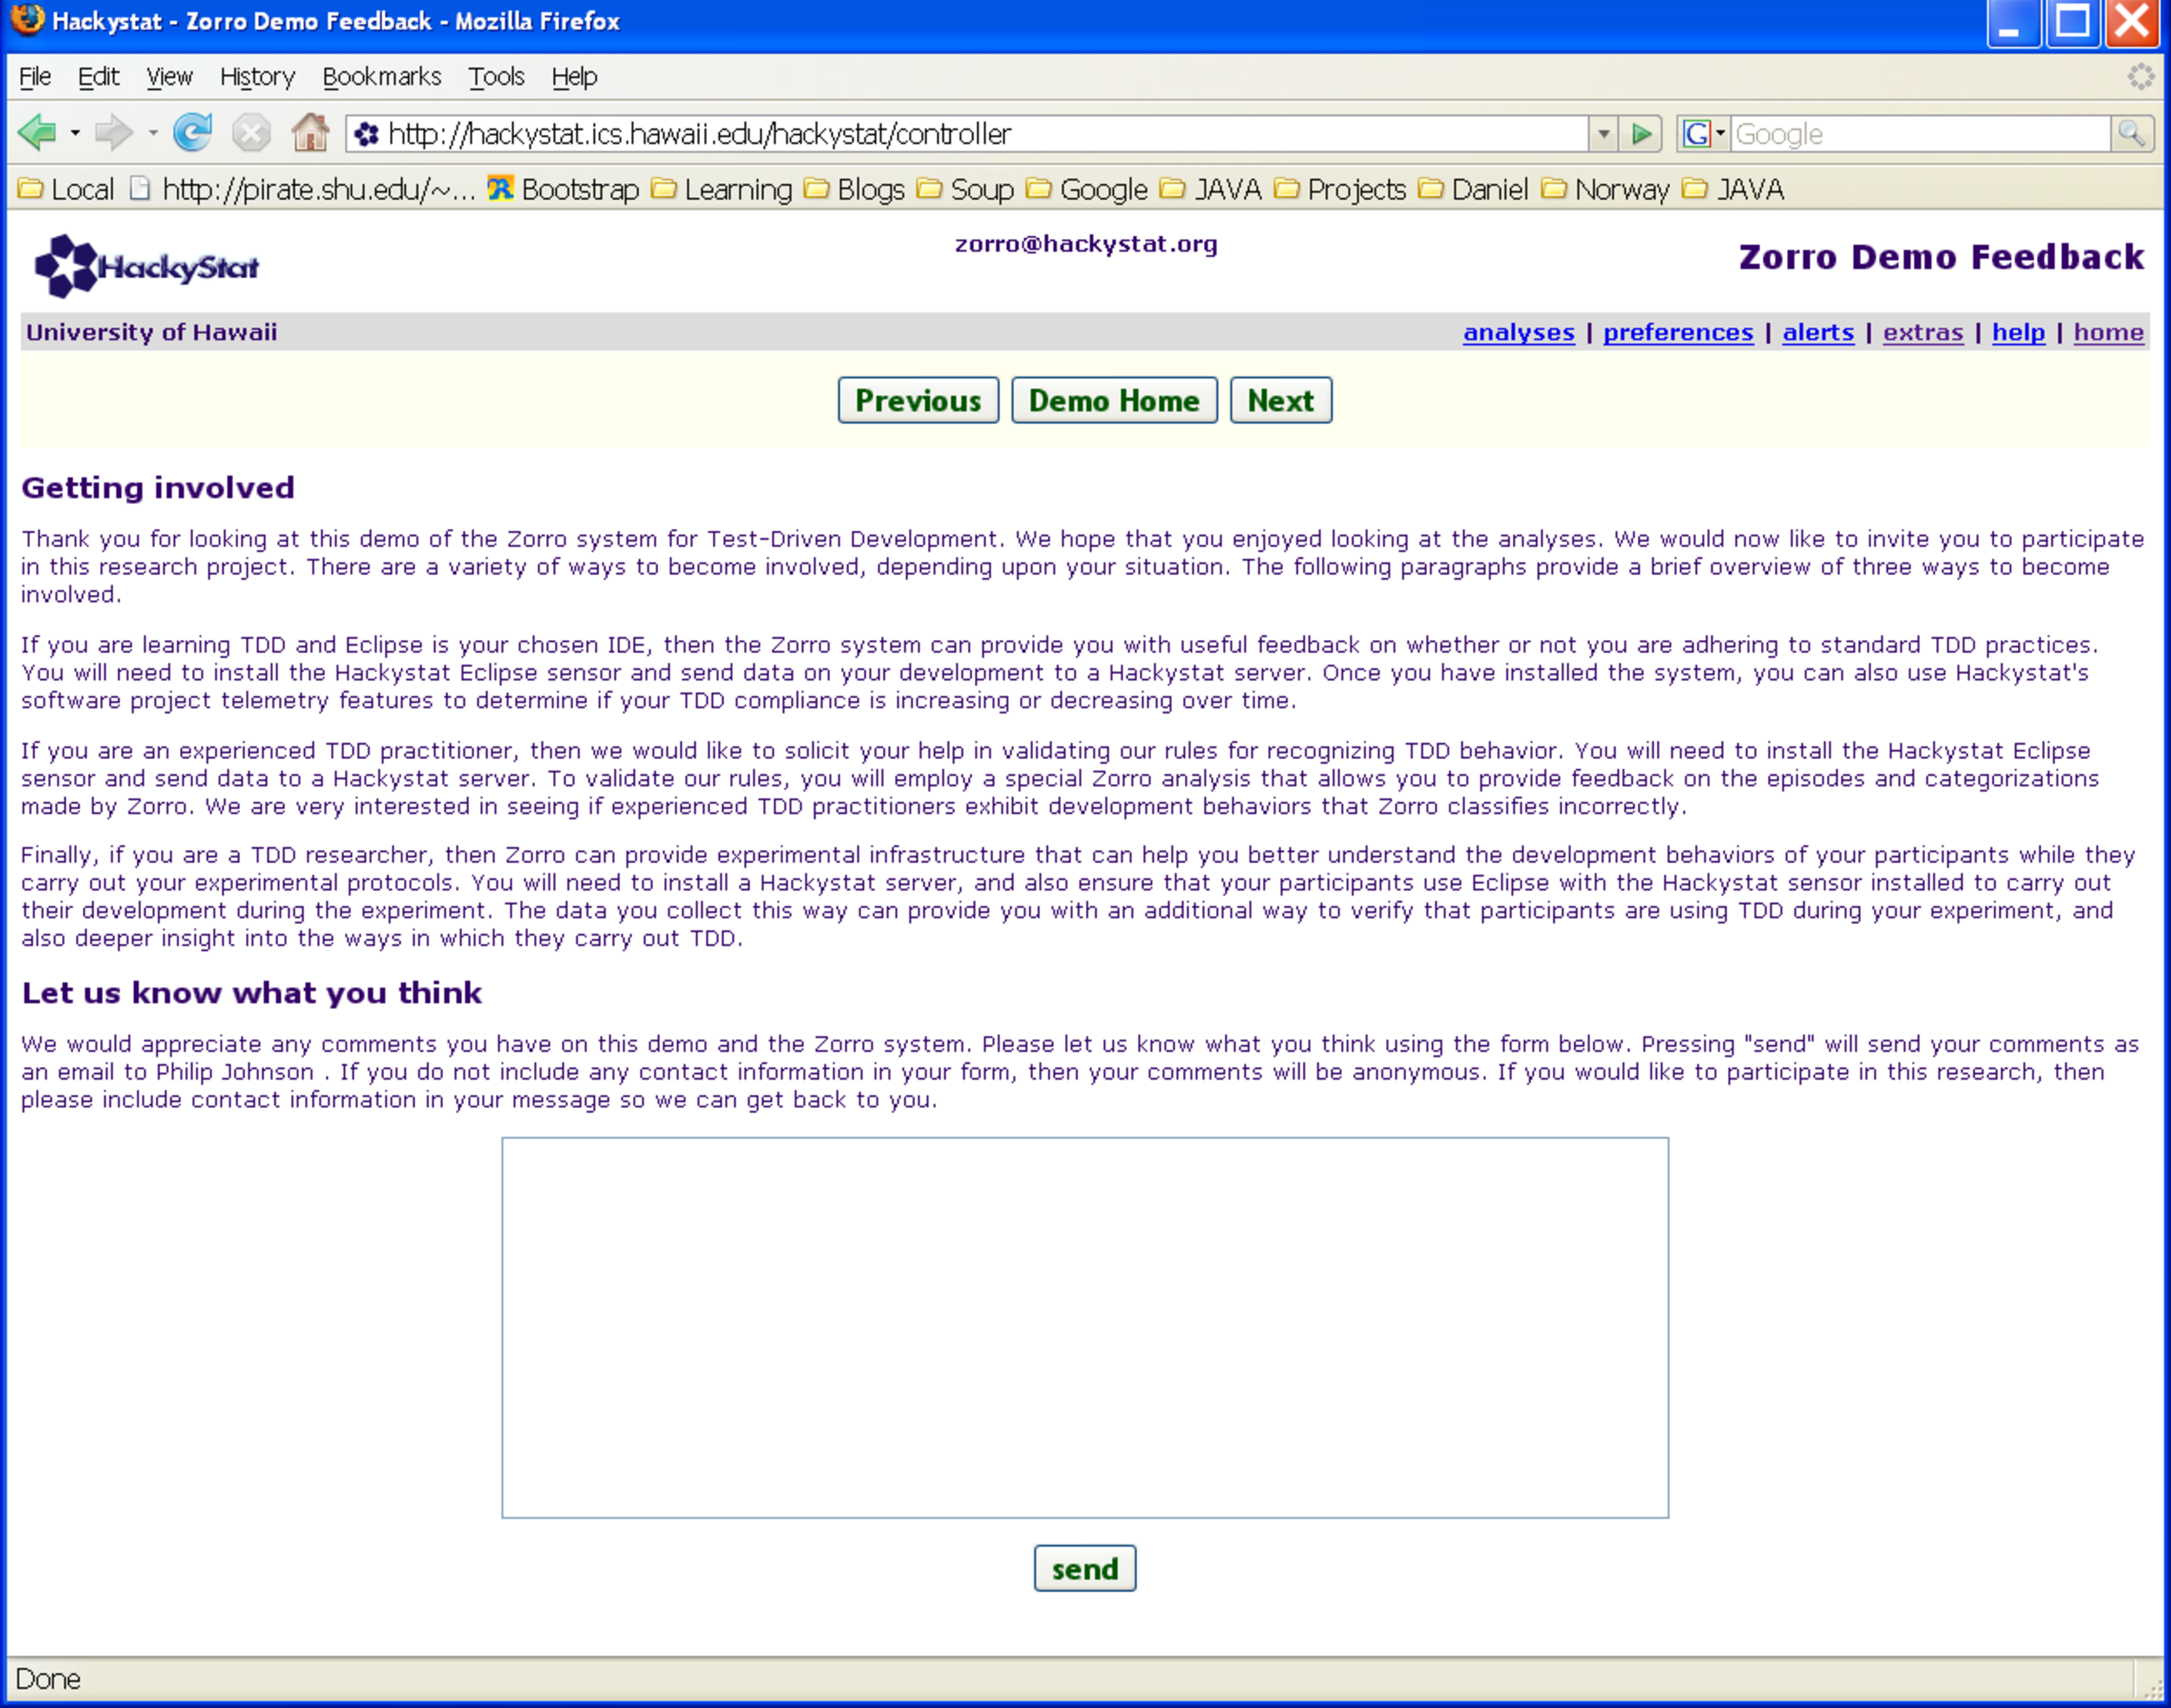
\includegraphics[width=0.85\textwidth]{figs/ZorroDemoP7}
  \caption{Zorro Demo Feedback}
  \label{fig:ZorroDemoP7}
\end{figure}

\end{enumerate}

\clearpage
\subsubsection{2006-11-07: Feedback from ISERN}
As the first step to find collaborative opportunity with researchers of TDD, we sent an RFC of Zorro Demo to the ISERN mailing list that contains researchers from worldwide who are interested in empirical software engineering research. On the same day we sent this collaboration solicitation email, Dr. Geir Hanssen and Dr. Tor Erlend F{\ae}gri from SINTEF ICT of Norway gave  very positive feedback on Zorro, and expressed that they were very interested in using Zorro in a comparative study between TDD and an existing Test-Last practice. 

They planned to conduct this study under the assistance from an European software company by harvesting data such as time spent for testing/coding, test code size/production code size etc. They were also interested in finding ways of validating any effect that the TDD-practice may have on product quality, speed of production, and also potentially on code quality (maintainability, code design-style and others). However, doing these was very hard in practice because the software company did not want to be disturbed when developers put maximum pressure on reaching the release deadline. As a result, collecting data became a problem in this already planned study. Thus, automated data collection became tempting and Zorro is such a tool that can bring immediate values to them.

Although Zorro was a good fit to this study, the software company used Visual Studio .NET rather than Eclipse, and the programming language was C\# rather than Java. A minimum set of sensor data types (See Table \ref{tab:Zorro.Sensors}) are required in order for Zorro to function. Unfortunately, the Visual Studio .NET senor was very premature and it can only collect a few of them. Thus, if we wanted to engage in this study, the most imperative task was to develop a Visual Studio .NET sensor that can collects necessary sensor data types. Moreover, the sensor had to be implemented and tested in a very short time frame since the software company planned to start the project in January 2007.

\subsection{Preparation}
\label{sec:Industry-Journal-Preparation}
With confidence in Zorro and our software development skills, we decided to participate in this collaborative industrial case study. The preparation tasks include implementation of the Visual Studio .NET sensor and installation of Hackystat.

\subsubsection{Visual Studio .Net Sensor Implementation}
We exchanged several emails with Dr. Hanssen to understand the company's development environment in December 2006. %It occurred to us that the Visual Studio .NET had a new version released in 2005, which has built in support of unit testing. 
With the help from Qin Zhang, another Ph.D student who was also my colleague in CSDL, I implemented the Visual Studio .NET sensor that was Zorro-compatible. After developing the sensor, I tested that Zorro can infer TDD development behaviors occurred in the IDE of Visual Studio .NET.  

\subsubsection{Hackystat Server Installation}
Zorro runs on the server-side of Hackystat. Foosball LLC provided a dedicated server for this study. Using Windows' Remote Desktop application, I logged into the server, installed and configured a Hackystat server for this case study in February 2007.

\subsection{Collaborative Research Activities}
In March 2007, the company launched both the TDD project and the Non-TDD project with 20 developers, twelve of which developed in TDD. I assisted developers installing the Visual Studio .NET sensor, which collected development activities in the background unobtrusively. Periodically, I analyzed the collected data and generated technique reports for Dr. Hanssen and the project manager regarding developers' development behaviors.

\subsubsection{2007-02-22: Sensor Installation Instruction}
Pertaining to the least possible interruption to the development process required by the participated company, I wrote a script to automate the sensor installation for developers. Figure \ref{fig:VSTE-Sensor-Script} illustrates the output from this script when a developer invoked this script. For each developer, I sent an individual email to him/her with customized installation instructions. Only one developer encountered difficult in installing the sensor due to his customization of the Windows user profile. I fixed this by patching the installation script. 

\begin{figure}[htbp]
  \centering
  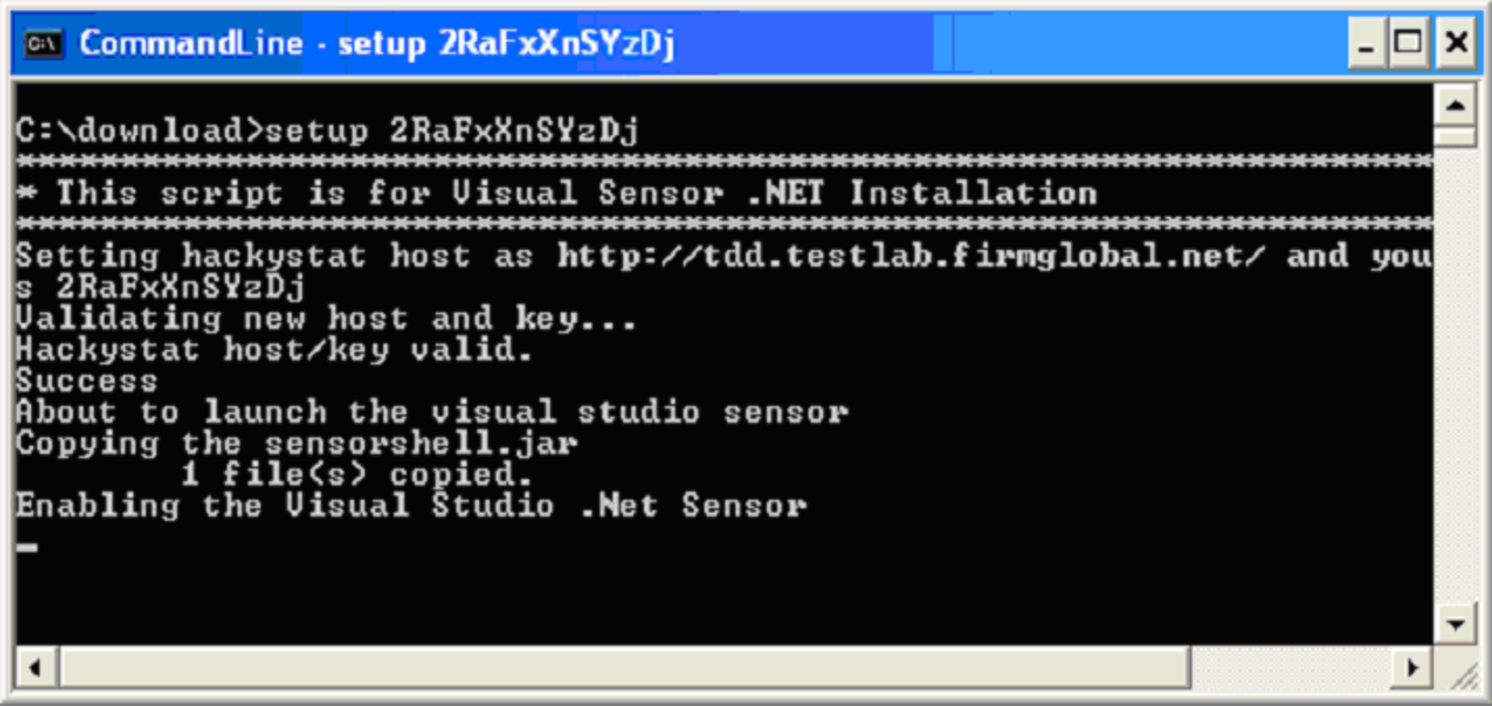
\includegraphics[width=1.0\textwidth]{figs/VSTE-Sensor-Script}
  \caption{Output of Visual Studio .NET Sensor Installation Script}
  \label{fig:VSTE-Sensor-Script}
\end{figure}

\subsubsection{2007-02-28: \#1  admin guide and sensor installation status}
The admin guide is a document for Dr. Hanssen and the project manager to use Hackystat and Zorro. This document covers following contents:
\begin{itemize}
\item Login as the administrator, 
\item Login as any developer,
\item Check sensor installation status (days with sensor data),
\item Check a developer's collected development activities,
\item Invoke the analyses described in the Zorro Demo.
\end{itemize} 
Following this guide, they can login as the administrator, check received data, define Hackystat projects, and invoke Zorro's analyses. 

I also summarized the sensor installation status based on data received on the server. According to this report, two developers successfully installed the sensor within a day after I sent the instructions to them. 

\subsubsection{2007-03-02: \#2 admin guide }
I updated the admin guide on March 2, 2007. According to this guide, some developers sent data to the Hackystat server. After observing the collected data, I registered projects for developers who installed the sensor so that the project manager can use Zorro to analyze their  development behaviors. 

When writing the sensor installation status report, I was surprised to find that none of developers invoked any unit tests. The project manager noticed this as well and asked us whether the sensor worked correctly with TestDriven.NET add-in. Unfortunately I never knew that developers ran tests with TestDriven.NET, a third-party add-in to the Visual Studio .NET. Later, we discovered that some emails from the project manager sent in January 2007 were discarded by the mail server of the University of Hawaii as SPAMs for unknown reasons. I configured my SPAM settings to allow emails sent from the software company, but I had to enhance the sensor to support TestDriven.NET quickly in order to continue this collaborative research. 

\subsubsection{2007-03-05: Support for TestDriven.Net and Sensor Upgrade}
TestDriven.NET was an open source project initially but turned into a proprietary Visual Studio add-in. It is not as extensible as the JUnit plugin of Eclipse so that a third-party observer can not listen to invocations of unit testing. Perhaps because Microsoft started a legal issue against him, the author of TestDriven.NET did not respond to my request for help. Soon I discovered an approach to capture and parse test running results from TestDriven.NET by observing the console output in Visual Studio .NET. After some extensive testing, I released a new Visual Studio .NET sensor for this collaborative industrial case study. %The Foosball LLC was very unhappy with this sensor upgrade but there was no alternatives if we wanted to continue this research. 

It was a little pity that the project manager was very unhappy with this update but there was no alternatives if we wanted to continue this research. As a result, some developers did not install this upgrade according to my observation of the server status. I addressed this issue in the following reports I wrote.

%, and we did not get further answers to our questions regarding their development process. 

\subsubsection{2007-03-20: \#3 sensor installation status}
I updated the sensor installation status report on March 20, 2007. According to this report, 20 developers fell into five groups:
\begin{itemize}
\item {\textbf{Group 1: Those who are successfully using the system}}

Four developers are sending coding and testing data regularly, indicating the sensor is installed and updated.

\item {\textbf{Group 2: Those who need to install the sensor}}

Four developers have not sent any data. They appear to have not installed the sensor at all or are not programming.

\item {\textbf{Group 3: Those who might have uninstalled the sensor}}

Four developers sent data at the beginning but have not sent any data recently. They have either uninstalled the sensor or are not programming.

\item {\textbf{Group 4: Those who might need to update the sensor}}

Four developers are sending coding data but not testing data. Either they are not testing, or have not updated the sensor.

\item {\textbf{Group 5: Those who apparently need to update the sensor}}

Four developers are sending coding data and testing data, but the test data lacks path information indicating the need to upgrade the sensor.

\end{itemize}

Because I conducted this study off-site, the above categorization of developers was only based upon my observation of data received on the Hackystat server. The project manager generously agreed to have developers update the sensor following my suggestions made in this report.  

\subsubsection{2007-04-14: \#4 introduction to the TDD telemetry analyses}

In the report I wrote on April 14, 2007, I introduced the TDD telemetry analyses (See Section \ref{sec:Zorro-Analysis-Telemetry}) to Dr. Hanssen and the project manager. In addition, I defined two Hackystat projects for them. One project was ``The-TDD-Project'' which includes all programmers who developed in TDD as project members, and the other project was ``The-NON-TDD-Project''.  With these two projects, they can invoke TDD telemetry analyses to compare the TDD project and the Test-Last project. A list of TDD telemetry analyses is in the following.

\begin{itemize}
\item {\textbf{DevTime-Chart:}} computes development time developers spent in the Visual Studio .NET environment.  
 
\item {\textbf{DevTime-Members-Chart:}} computes and plots all project members' development time spent in the Visual Studio .NET environment.

\item {\textbf{DevTime-TotalProductionTest-Chart:}} computes and illustrates total development time, the portion on coding, and the portion on testing. 
 
\item {\textbf{EpisodeDurationAverage-Chart:}} illustrates the average episode durations.

\item {\textbf{TDD-Percent-Chart:}} reports the percentage of a project's TDD compliance.
 
\item {\textbf{TDD-All-Members-Chart:}} reports and compares project members' TDD compliance.

\item {\textbf{TDDPercent-And-DevTime-Chart:}} combines the TDD compliance percentage and development time to a given project.
\end{itemize}

Basically this report opened a door to Zorro and Telemetry for Dr. Hanssen and the project manager. With the sensor data collected from developers, Zorro can be used to not only infer developers' TDD development behaviors but also conduct comparative study between TDD and Non-TDD.  

According to feedback received from Dr. Hanssen regarding this report, the number of programmers producing data was disappointing, and he would contact the project manager directly for possibility to improve it. However, he viewed this study as a pilot and planned to replicate it in another software company, which might have a better start and more complete data. Also, other researchers are interested in Zorro's automation of data collection and development behavior inference. 

\subsubsection{2007-05-04: \#5 Comparison Between TDD and Test-Last Projects}
I used Zorro's TDD telemetry analyses to compare development behaviors between the TDD project, and the Test-Last project and wrote a technique report on May 4, 2007. The main points included in this reports are:

\begin{itemize}
\item {\textbf{TDD-Percent-Chart (by development time)}}

The ``TDD-Percent-Chart'' telemetry analysis computes and plots percentages of development time that developers complied to TDD based upon Zorro's inference. Partially due to the imperfect sensor installation, developers did not comply to TDD faithfully in this study. The compliance percentage was 5\% at the best on the weekly basis.

Living far from developers who participated in this study, I did not have the capabilities to investigate causes for the low TDD compliance rate. Perhaps developers did not have the necessary skills to use TDD on their development tasks, or they modified TDD according to their needs. 

\item {\textbf{TPRatio-DevTime-Chart}}

The ``TPRatio-DevTime-Chart'' telemetry analysis is a metric for measuring effort developers devoted to testing. It was interesting to note that developers who were in TDD project evenly divided their effort on testing and production code. On the contrary, developers in the Test-Last project did not test much at the beginning but gradually caught up unit testing. 

\item {\textbf{DevTime-TotalProductionTest-Chart}}

The ``DevTime-TotalProductionTest-Chart'' telemetry chart analysis plots cumulative effort spent on test and production code. According to this analysis, the TDD project had larger growth rate of test code while the Test-Last project had larger growth rate of production code. 

\item {\textbf{DurationAverage-Chart}}

The ``DurationAverage-Chart'' telemetry analysis illustrates how frequently developers invoked unit tests. Interestingly, the episode durations average of the two projects are far longer than 10 minutes.  

\end{itemize}

In addition to the telemetry report, I updated the sensor installation status with development time and T/P ratio for each developer. After reading this report, Dr. Hanssen were more concerned about the legitimacy of the data rather than the hypotheses I claimed regarding the development process. Unfortunately, the project manager concentrated on the software development and did not respond to this report. 

\subsubsection{2007-05-25: \#6 Comparison Between TDD and Test-Last Projects}
Based on the report I wrote on May 25, 2007, developers in the Test-Last project started putting more effort on testing than effort on production code, in contrast developers in the TDD project evenly divided their effort on testing. 

\subsection{Phone Interview with the Researcher}
By the time I write this chapter, developers in Foosball LLC are still working on the software to make the next release. In this research, I installed and configured a Hackystat server for them, developed the Visual Studio .NET sensor, managed the Hackystat server, and wrote six technique reports for the researcher and the project manager. After four months collaboration, Professor Philip Johnson and I interviewed the researcher on July 3, 2007. Table \ref{tab:InterviewStructure} lists the structure of this interview.
\begin{table}[!ht]
\centering
\caption{Structure of the Interview with the Researcher}
\begin{tabular}{|l|l|} \hline
Interviewer & Hongbing Kou, Philip Johnson  \\ \hline
Interviewee & Geir Hanssen \\ \hline
Instrumentation & Voice Recorder \\ \hline
Method      & Phone \\ \hline
Time        & 9PM July 3, 2007 \\ \hline
Length      & 45 minutes \\ \hline
Location    & Collaborative Software Development Laboratory \\ \hline
\end{tabular}
\label{tab:InterviewStructure}
\end{table}

In the interview, we mainly focused on the experiment details behind the scene as well as the researcher's experience regarding this collaborative research. 

\begin{itemize}
\item {Research Background}

It is interesting to note that the Foosball LLC was not specially recruited to participate in this comparative study of TDD. The company worked with Dr. Hanssen before on studying Evo Agile, an agile process that the company has adopted. For whatsoever reason, the company decided to include TDD in its software process and so this case study was initiated. After seeing the Zorro Demo, Dr. Hanssen suggested that they use Zorro for data collection in this study. Because of the unobtrusiveness of Zorro's data collection, the Foosball LLC agreed to have its process instrumented. 

\item {TDD Conformance}

The TDD compliance percentage of this study was very low according to Zorro's inference. However, probing the development process to understand the situation was impossible for me and Dr. Hanssen as well at this moment. Typically, the Foosball LLC has good reputation in complying to what they agreed to, but meeting the deadline has the top priority. It is worthwhile to note that Evo Agile, the software process that the company is using, has tight and well scheduled development activities. TDD is an extra addition to the process, which might help to explain why the project manager did not respond to our requests for understanding their software process.  

\item {Concerns on Sensor Installation}

In the \#3 report of ``Sensor Installation Status Update'', I described the sensor installation status after a month's deployment. We were confident that 4 developers successfully installed and updated the sensor as requested, but not sure what happened to the rest developers. A real problem occurred in this study was from the TestDriven.NET plugin. I had to enhance the Visual Studio .NET sensor rapidly, and in turn, developers had to update the sensor shortly after installation. Likely some developers gave up the sensor although upgrading the sensor was a trivial task from our perspective.

As concerned as we were on this problem, Dr. Hanssen said that he will call each developer after the project is released. A questionnaire will be designed regarding the development process, sensor installation and Zorro's inference results. 

\item {Experience on Collaborative Research with Industry}

Collaborative research with industry in generally is hard. In this research, the project manager did not respond to Zorro's inference regarding their development process. To the industrial participants, meeting deadlines of project releases have much higher priority than engaging in research activities. In Dr. Hanssen's opinion, this is just the way it is, and as researchers, we have to adopt this. A few key points he described in the interview were:
\begin{itemize}
\item This study is a training to use tools such as Zorro that automate the data collection. 
\item What we can do better in the future is to let developers install Zorro, make sure that it works.
\item He is interested in conducting more of this kind of study. Other companies are interested in TDD too. 
\end{itemize}
\end{itemize}

\section{Conclusions}
\label{sec:Industry-Conclusions}

This study shows that Zorro can support empirical research of TDD. The automation of data collection makes it possible for researchers to collect data without interrupting the development process. It provides supporting evidence to the research question Q3a, but it also shows that installing sensors to enable automated data collection can be a challenging task to the participants. 

\section{Chapter Summary}
\label{sec:Industry-Summary}

This chapter introduces the industrial case study I collaboratively conducted with Dr. Hanssen, a TDD researcher, and an European software company. In this collaborative study, I provided technique support of Hackystat and Zorro. %Dr. Hanssen planned to use the collected data as supplemental research materials to survey developers after the project is finished. Additionally, he wanted to replicate this study within other software companies that are interested in adopting TDD. 

The lessons I learned from this study are:
\begin{itemize}
\item{\textbf{Pilot}}

Pilot is a must for studies to be conducted in the industrial settings. Participants are very precious resources, and if possible, all the research activities should be pilot tested beforehand. Otherwise, it will be very easy to make mistakes that may blow up the research opportunity. %that has been planned for months. 

\item{\textbf{On-site}}

Another lesson I learned from this study is that case studies should be conducted on-site instead of off-site. Responding to requests from researchers is more or less a burden to the participated companies. In case when the schedule is tight, participants may ignore requests from researchers. To effectively conduct case studies, the researchers can get maximum input from participated companies if they can go to the field to conduct research. 

\item{\textbf{Periodical Sensor Installation Status Check}}

With automated data collection, researchers may tempt to focus on other research areas instead of data collection. The lesson we learned from this research is that periodically checking data collection is necessary because many things can go wrong. For example, some unit testing activities were not collected at the beginning of this industrial case study. Also, developers might silently decline the request to instrument their development processes with sensors.

\item{\textbf{The Author's Involvement}}

Finally, so far my involvement is still necessary in order to use Zorro in the evaluation case studies of TDD. In this industrial case study, I deployed Zorro to the site, assisted developers installing the sensor, analyzed the data, and wrote analysis reports for the researcher. For those who have no prior experience to Hackystat and Zorro, adopting Zorro in the empirical evaluation studies might be hard. 

\end{itemize}
